\documentclass[
  12pt,				    % tamanho da fonte
  openright,			% capítulos começam em pág ímpar (insere página vazia caso preciso)
  oneside,			  % para impressão em recto e verso. Oposto a oneside
  a4paper,			  % tamanho do papel. 
  hyphens,
  chapter=TITLE,  % títulos de capítulos convertidos em letras maiúsculas
  section=TITLE,  % títulos de seções convertidos em letras maiúsculas
  english,			  % idioma adicional para hifenização
  french,				  % idioma adicional para hifenização
  spanish,			  % idioma adicional para hifenização
  brazil				  % o último idioma é o principal do documento
]{iftex}

% Importa as macros do projeto
%% Macros de dados do documento
\autor{Nícolas Dezan dos Santos}
\titulo{AUTOMAÇÃO DE UM MALTEADOR LABORATORIAL: DESENVOLVIMENTO DE FIRMWARE E APLICATIVO PARA CONTROLE DE PROCESSOS}
\instituicao{Instituto Federal do Espírito Santo}
\newcommand{\campus}{Campus Vila Velha}
\newcommand{\imprimircampus}{\campus}
\curso{Curso de Química Industrial}
\local{Vila Velha-ES}
\data{2025}


\tipotrabalho{Trabalho de Graduação}
\preambulo{Trabalho de Conclusão de Curso apresentado à Coordenadoria do Curso de Química Industrial do
Instituto Federal de Educação, Ciência e Tecnologia do Espírito Santo, como requisito parcial para a obtenção do título de Químico Industrial.}

\orientador[Orientador][Prof. Dr.]{Ernesto}[Corrêa Ferreira]{Instituto Federal do Espírito Santo}
\coorientador[][]{}[]{}

\examinadori{Profa. Dra. Fulana de Tal}{Instituto Federal do Espírito Santo}{Examinadora} % DEPOIS
\examinadorii{Prof. Dr. Cicrano de Tal}{Instituto Federal do Espírito Santo}{Examinador} % DEPOIS

\approvaldate{32}{Dezembro}{2999} % DEPOIS

% Palavras-chaves
\palavraschave{Automação}[Malteação][Firmware][Engenharia de Alimentos][Controle de Processos]
\keywords{keyword 1}[keyword 2][keyword 3][keyword 4][keyword 5]

% Ficha catalográfica
\fichabiblioteca{
    Dados Internacionais de Catalogação-na-Publicação (CIP) \\
    (Biblioteca Nilo Peçanha do Instituto Federal do Espírito Santo) % Vish
}
\fichaautor{Elaborada por XXXXXXXXXXXXXXXXXXXXX – CRB-X/ES - XXX}
\fichatags{
    1. Redes neurais (Computação).  2. Expressão facial – Processamento de dados. 3. Sistemas de reconhecimento de padrões. 4. Processamento de imagens – Técnicas digitais. 5. Percepção de padrões. 6. Engenharia Elétrica. I. XXXXXXXX, XXXXXXXXXX XXXXXXXXXX.  II. Instituto Federal do Espírito Santo. III. Título.
}

\cutter{X999y}
\cdd{000.00}
\selectlanguage{brazil}

% Arial (para usar times-new-roman, comente as três linhas abaixo)
\usepackage{helvet}
\renewcommand{\familydefault}{\sfdefault}
\renewcommand{\ABNTEXchapterfont}{\bfseries}
% Comandos para revisar o texto
\usepackage{easyReview} 


%% Elementos opcionais
\editardedicatoria{\input{pre_textuais/dedicatoria}}
\editaragradecimentos{\input{pre_textuais/agradecimentos}}
\editarepigrafe{\input{pre_textuais/epigrafe}}


%% Listas [Siglas e Simbolos]
\editarlistasiglas{\input{pre_textuais/siglas}}
\editarlistasimbolos{\input{pre_textuais/simbolos}}

% Novos comandos
\newcommand{\ie}{\textit{i.e. }}
\newcommand{\eg}{\textit{e.g. }}



\begin{document}



  % --------------------------------------------------- %
  % CAPAS                                               %
  % --------------------------------------------------- %
  % CAPA E FOLHA DE ROSTO
  \capas
  \imprimircapa
  \imprimirfolhaderosto
  % \imprimirfichacatalografica
  % \includepdf[pages=-]{pre_textuais/ficha.pdf}

  % --------------------------------------------------- %
  % ELEMENTOS PRÉ-TEXTUAIS                              %
  % --------------------------------------------------- %
  % APROVAÇÃO, DEDICATÓRIA, AGRADECIMENTOS, EPÍGRAFE
  \pretextual
  % \imprimiraprovacao
  % \includepdf[pages=-]{pre_textuais/aprovacao.pdf}
  % \imprimirdedicatoria
  % \imprimiragradecimentos
  % \imprimirepigrafe
  
  % RESUMO - PT/EN
  % RESUMO - PT
\begin{resumo}
  \vspace{-15pt}
  
  A malteação é uma etapa crítica na produção de cerveja, exigindo o controle rigoroso de variáveis como temperatura, umidade e tempo ao longo das fases de maceração, germinação e secagem. Em ambientes acadêmicos, a ausência de equipamentos acessíveis e confiáveis limita o desenvolvimento de pesquisas nesta área. Este trabalho apresenta o desenvolvimento de um sistema de automação baseado no microcontrolador ESP32, com firmware programado em MicroPython e um aplicativo Android desenvolvido em Kotlin, capaz de monitorar e controlar o processo de malteação em laboratório. O sistema permite a configuração remota dos parâmetros de processo e o monitoramento em tempo real por meio da comunicação via Bluetooth Low Energy (BLE). A arquitetura do firmware foi estruturada com tarefas assíncronas independentes para controle de sensores, atuadores e etapas do processo. O aplicativo Android adota a arquitetura moderna em camadas (data, domain, presentation) com interface responsiva em Jetpack Compose, proporcionando usabilidade e modularidade. Os códigos desenvolvidos estão disponibilizados em repositórios GitHub, com o objetivo de promover reprodutibilidade e facilitar a adoção por outros pesquisadores. A solução proposta visa atender às demandas do LACEMP-IFES por uma plataforma de baixo custo e alta eficiência, contribuindo para a pesquisa aplicada em tecnologia de alimentos e automação de processos.

  Palavras-chave: \palavraschaveemlinha
\end{resumo}


% RESUMO - EN
\begin{resumo}[Abstract]
  \vspace{-15pt}
  
  \begin{otherlanguage*}{english}
    Malting is a critical stage in beer production, requiring strict control of variables such as temperature, humidity, and time during the steeping, germination, and kilning phases. In academic environments, the lack of accessible and reliable equipment limits research progress in this field. This work presents the development of an automation system based on the ESP32 microcontroller, with firmware programmed in MicroPython and an Android application developed in Kotlin, capable of monitoring and controlling the malting process in a laboratory setting. The system enables remote configuration of process parameters and real-time monitoring via Bluetooth Low Energy (BLE) communication. The firmware architecture was structured with independent asynchronous tasks to handle sensors, actuators, and process stages. The Android application adopts a modern layered architecture (data, domain, presentation) with a responsive interface built using Jetpack Compose, providing usability and modularity. The developed code is publicly available on GitHub, aiming to promote reproducibility and facilitate adoption by other researchers. The proposed solution addresses the demands of LACEMP-IFES for a low-cost and efficient platform, contributing to applied research in food technology and process automation.
  
  Keywords: \inlinekeywords
\end{otherlanguage*}
\end{resumo}
  
  % LISTAS E SUMÁRIO
  % \imprimirlistafiguras
  % \imprimirlistatabelas
  % \imprimirlistaquadros
  % \imprimirlistasiglas
  % \imprimirlistasimbolos
  \imprimirsumario

  % --------------------------------------------------- %
  % ELEMENTOS TEXTUAIS                                  %
  % --------------------------------------------------- %
  \textual
  \graphicspath{{figuras/}}   
  \chapter[Introdução]{Introdução}

O malte é um produto de extrema importância para diversos setores industriais, com ele sendo o principal insumo na produção de cerveja, onde fornece açúcares fermentáveis, cor e aroma à bebida. No setor cervejeiro, o malte de cevada é o mais utilizado; no entanto, há um crescente interesse em pesquisas que buscam desenvolver malte a partir de outros grãos, como arroz, milho e trigo, visando atender demandas específicas, como a produção de cervejas livres de glúten \cite{CECCARONI2019}. Além disso, o malte tem ganhado destaque como ingrediente funcional na indústria alimentícia, sendo utilizado, por exemplo, na fabricação de pães, devido às suas propriedades nutricionais \cite{KOISTINEN2020}.

A produção de malte, no entanto, enfrenta desafios significativos, especialmente em climas quentes, onde o controle preciso de temperatura, umidade e tempo, durante as etapas de maceração, germinação e secagem, é crucial para garantir a qualidade do produto \cite{KOVALOVA2024}. O controle desses parâmetros torna a malteação um processo complexo, exigindo equipamentos especializados e sistemas automatizados para otimizar a produção. No contexto acadêmico e de pesquisa, a falta de equipamentos acessíveis e confiáveis para malteação em laboratório limita o desenvolvimento de estudos e inovações nesta área, evidenciando a importância de soluções de baixo custo.
% A base dessa minha afirmação "forte" foram minhas pesquisas mais diretas por equipamentos, que normalmente são industriais. Essa é a forma que encontrei para justificar o trabalho, não sei se foi a melhor abordagem, mas parece funcionar. - Nicolas

Nesse contexto, um dos principais desafios enfrentados é a falta de equipamentos que permitam a malteação controlada em laboratório, comprometendo a precisão e a reprodutibilidade dos experimentos. Durante uma iniciação científica (IC), foi desenvolvido um protótipo inicial (\autoref{fig:malteador}), não finalizado, restando completar a montagem física e desenvolver o sistema de controle e automação. O presente trabalho dá continuidade à IC ao propor uma solução de \textit{software} responsável por garantir que o processo de malteação ocorra adequadamente. 
% A minha intenção é que essa última frase exponha os objetivos do trabalho. - Nicolas

\begin{figure}[ht]
    \centering
    \caption{Protótipo desenvolvido durante a IC. (A) Interface, placa de desenvolvimento e relés das válvulas; (B) Relé de estado sólido; (C) Parafuso de revolvimento; (D) Entrada de ar; (E) Entrada de água; (F) Saída de água; (G) Sensor de dióxido de carbono, umidade e temperatura.}  
    \label{fig:malteador}
    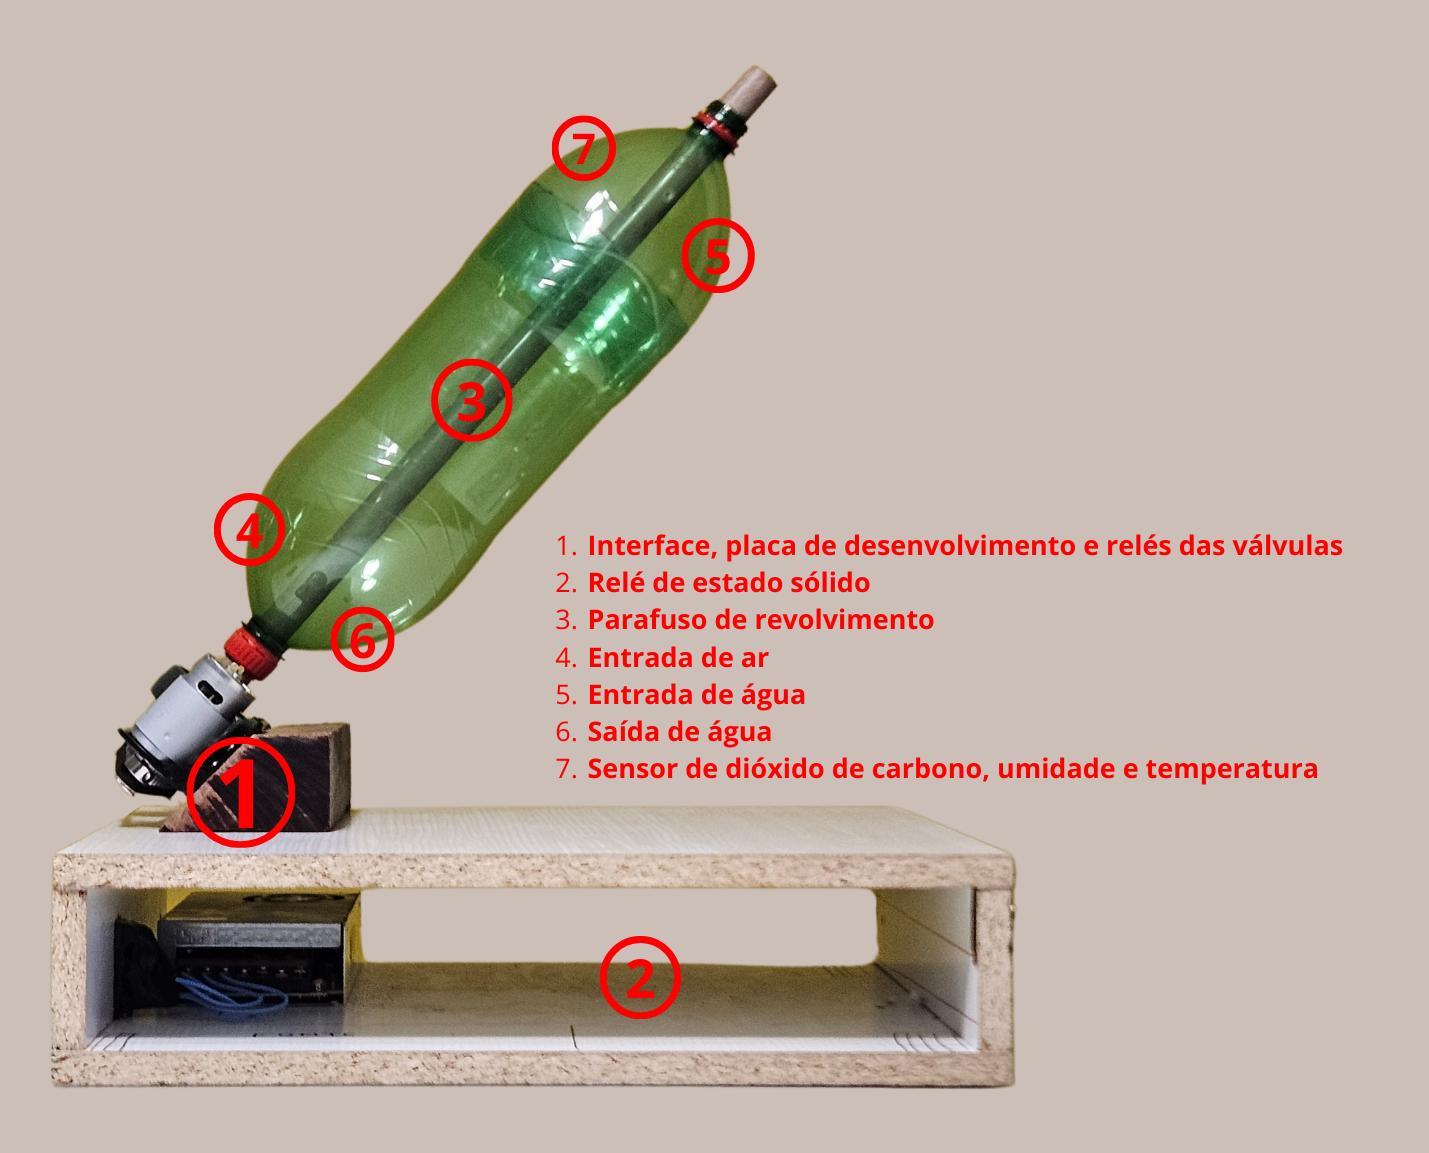
\includegraphics[width=0.8\textwidth]{Vista Lateral do Malteador.png}

    {\centering\footnotesize Fonte: Autoria própria.\par}
\end{figure}

A proposta visa o desenvolvimento de um sistema (\autoref{fig:esquemaeletronico}) baseado no microcontrolador ESP32-C3, da fabricante chinesa Espressif Systems, integrado com um aplicativo Android. Esse microcontrolador foi escolhido por sua relação custo-benefício, capacidade de processamento e suporte a tecnologias de comunicação como Bluetooth e Wi-Fi \cite{rodrigues2021controle, santos2019sistema}. Para seu firmware, optou-se pela linguagem MicroPython, que oferece uma curva de aprendizado suave e é bastante utilizada em projetos de prototipagem rápida e Internet das Coisas (IoT) \cite{TOLLERVEY2017, brito2020automaccao}. Já o aplicativo Android foi desenvolvido em Kotlin, linguagem oficial para o desenvolvimento Android \cite{sempreupdate_kotlin_2020}. A comunicação entre o firmware e o aplicativo é realizada via Bluetooth Low Energy (BLE), uma tecnologia de baixo consumo energético e amplamente disponível em dispositivos móveis \cite{heydon2012bluetooth}, permitindo a configuração remota e o monitoramento em tempo real dos parâmetros operacionais. Além disso, a documentação dos softwares desenvolvidos pode servir como referência para outros estudos envolvendo IoT dentro do IFES, especialmente no que se refere à integração entre ESP32 e Android.
% Adicionei referências a esse parágrafo. - Nicolas

\begin{figure}[ht]
    \centering
    \caption{Esquema eletrônico do malteador desenvolvido durante a IC: (A) relés para atuação das válvulas; (B) relés para atuação do motor e da resistência elétrica; (C) sensor de umidade, temperatura e dióxido de carbono; (D) painel LCD; (E) botão de emergência; (F) microcontrolador ESP32}
    \label{fig:esquemaeletronico}
    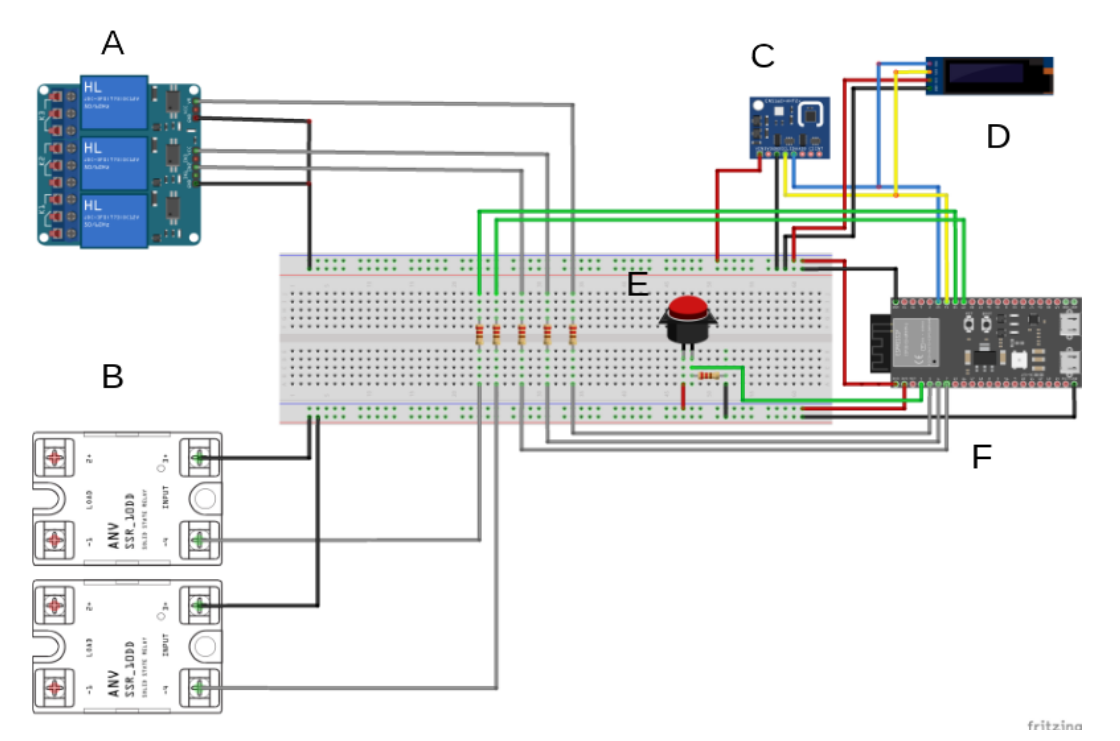
\includegraphics[width=0.8\textwidth]{esquemaeletronico.png}

    {\centering\footnotesize Fonte: Autoria própria.\par}
\end{figure}


Este trabalho surge a partir da demanda do Laboratório de Análises de Cerveja e Matérias-Primas (LACEMP), que busca iniciar estudos experimentais sobre o processo de malteação. A ausência de um equipamento adequado e acessível para pesquisas acadêmicas motivou o desenvolvimento de um sistema que permita monitorar e controlar as variáveis do processo de forma precisa e reprodutível. 

Por fim, a automação proposta busca simplificar a operação do equipamento e fornecer dados estruturados sobre o processo, facilitando futuras análises e ajustes nos experimentos conduzidos no LACEMP. Com isso, espera-se que esta solução de baixo custo promova avanços tanto na pesquisa acadêmica quanto no desenvolvimento de tecnologias acessíveis para a indústria cervejeira e áreas afins.
  \chapter[Referencial Teórico]{Referencial Teórico}

\section{O Processo de Malteação}

A malteação é um dos processos fundamentais na indústria cervejeira, responsável pela conversão do grão cru em um ingrediente essencial para a produção de cerveja. Esse processo ocorre em três etapas principais: maceração, germinação e secagem. Essas etapas são fundamentais para a produção de malte base: um malte que possui uma boa quantidade de enzimas e estoques de amido \cite{BRIGGS2004,CENCI2021}. Além disso, pode-se considerar uma quarta etapa no processo: a torrefação, que ocorre após a secagem e produz um malte especial no lugar de um malte base. Maltes especiais são conhecidos por serem formados com bastante influência das reações de Maillard \cite{COGHE2004}. A complexidade desse processo se dá no fato da manipulação de um organismo vivo, o grão, que exige controle rigoroso de suas condições de crescimento para se tornar um produto viável para comercialização \cite{MALLETT2022}. Além disso, em condições inadequadas de malteação, podem ocorrer ataques microbiológicos de diversas espécies, incluindo \textit{Fusarium sp.}, \textit{Penicillium} e \textit{Aspergillus genera} \cite{LUARASI2016}.

\subsection{Maceração}

Durante a maceração, com a submersão do grão em água, ocorre a liberação de hormônios e enzimas que darão início ao crescimento e desenvolvimento do grão \cite{LEWIS2012}. O teor de água no grão cresce rapidamente após o início dessa primeira etapa, que ocorre em duas fases distintas: uma inicial, em que o embrião e o escutelo absorvem água rapidamente, e uma segunda fase, mais lenta, em que o endosperma é gradualmente hidratado. Esse processo é crucial para a ativação de enzimas como a amilase, a ribonuclease e a fosfatase, que desempenham papeis essenciais na modificação do grão \cite{REYNOLDS1966}. Também é crucial que o oxigênio seja fornecido ao mesmo tempo em que o dióxido de carbono é eliminado dos grãos. O aumento da umidade intensifica o metabolismo do grão, elevando sua taxa respiratória, ou seja, mais oxigênio é requerido \cite{KUNZE1996}. Por isso, a presença de tanques de maceração que bombeiam ar através dos grãos submersos é frequente nas produções de larga escala \cite{CENCI2021}. Mas, muitos estudos ainda investigam os impactos de se trabalhar com ciclos de períodos secos e submersos, especialmente, quando se busca viabilizar novas variedades de grãos para a malteação \cite{MAYER2014,TURNER2019}.

\subsection{Germinação}

Ao fim da maceração, que pode durar até 72 horas, o teor de umidade dos grãos chega a aproximadamente 45\%, e as radículas tornam-se visíveis, indicando o momento adequado para o início da germinação. Essa segunda etapa é caracterizada por um elevado nível metabólico nos grãos, com a ocorrência de transformações bioquímicas essenciais para o processo de malteação \cite{MALLETT2022}. Do ponto de vista do malteador, a duração da germinação deve ser cuidadosamente controlada, pois um período insuficiente ou excessivo pode comprometer a qualidade do malte. Se a germinação for muito curta, as transformações necessárias nos grãos não ocorrerão de forma adequada. Por exemplo, as enzimas não conseguirão degradar completamente as paredes celulares proteicas que envolvem o amido, tornando-o menos disponível para as etapas subsequentes do processo cervejeiro \cite{FOX2009}. Por outro lado, uma germinação prolongada pode levar ao esgotamento excessivo dos nutrientes do grão visando o crescimento da planta, afetando negativamente o produto final \cite{LEWIS2012}.

Durante a germinação, a ativação de enzimas hidrolíticas desempenha um papel essencial na modificação do grão.As $\beta$-glucanases promovem a degradação dos $\beta$-glucanos presentes na parede celular do endosperma, substâncias estas que são indesejadas no processo cervejeiro em altas concentrações \cite{LEWIS2012}. Paralelamente, proteases hidrolisam a matriz proteica que envolve os grânulos de amido, liberando pequenos peptídeos e aminoácidos \cite{FOX2009,GUPTA2010}. Já a conversão do amido é mediada por enzimas amilolíticas,sendo a $\alpha$-amilase responsável pela quebra aleatória das ligações $\alpha$-1,4-glicosídicas e a $\beta$-amilase pela liberação de maltose, um dos principais açúcares fermentáveis do processo cervejeiro \cite{GUPTA2010,MALLETT2022}. Em essência, o grão cru entra no processo com compostos de alto peso molecular e, ao fim da malteação, gera como produto um malte com compostos de baixo peso molecular e boa concentração de enzimas \cite{KUNZE1996}. Essa transformação, que ocorre principalmente na germinação, é o que torna o malte indispensável para o processo cervejeiro \cite{CENCI2021}.

\subsection{Secagem}

Quando a germinação atinge o tempo otimizado para promover as melhores transformações, inicia-se a etapa de secagem. Nessa fase, de acordo com \apudonline{GRIFFITHS1992}{WOFFENDEN2002}, os grãos são desidratados por até 30 horas, o que resulta em um malte base de fácil manuseio e adequado para armazenamento. Além da redução da umidade para aumento da estabilidade do produto final, a secagem promove o desenvolvimento de aromas desejados e de coloração no malte \cite{BAMFORTH2003}. Apesar disso, se a intenção é produzir um malte base, a temperatura não pode ser excessiva, com o fim de preservar as enzimas, como as amilases, no produto final \cite{LEWIS2012}.Outra questão benéfica é que a secagem elimina boa parte dos microorganismos que cresceram de forma indesejada durante os processos anteriores \cite{DOUGLAS1988, PETTERS1988}. 


\section{Importância do controle de variáveis na malteação}

\subsection{Controle de temperatura}

O controle da temperatura durante a germinação é essencial para minimizar perdas causadas pelo crescimento excessivo das radículas e do embrião da planta, evitando o consumo desnecessário dos estoques de amido do grão \cite{PITZ1990, MALLETT2022}. Além disso, a temperatura influencia diretamente a atividade enzimática e a degradação de componentes estruturais do grão. Um estudo conduzido por \citeonline{BAXTER1980} avaliou os efeitos da maceração em uma temperatura superior à faixa usual de 12-16 $^{\circ}$C, chegando a 30 $^{\circ}$C. Os resultados indicaram que temperaturas elevadas comprometem a atividade enzimática e reduzem a eficiência da degradação de $\beta$-glucanos e proteínas, afetando negativamente a qualidade do malte.

Outro fator crítico relacionado à temperatura é o crescimento microbiológico. Segundo \citeonline{TANGNI2002}, temperaturas mais altas na malteação favorecem a proliferação de \textit{Aspergillus clavatus}, um fungo produtor de micotoxinas. A contaminação microbiológica ocorre predominantemente durante a germinação, mas também pode ser observada ao final da maceração \cite{PETTERS1988}. Dessa forma, a manutenção de temperaturas controladas entre 12 e 22 $^{\circ}$C durante as etapas de maceração e germinação é fundamental não apenas para garantir a qualidade do malte, mas também para assegurar a segurança sanitária do processo \cite{TANGNI2002}.

\subsubsection{Controle de temperatura na secagem}

Na etapa de secagem, o controle da temperatura desempenha um papel crucial em dois aspectos principais: garantir que o malte atinja a umidade adequada para armazenamento e determinar o tipo de malte produzido \cite{KUNZE1996}. A secagem ocorre, geralmente, em múltiplas fases, seguindo uma rampa de temperatura. Os valores típicos variam na faixa de 50 a 110 $^{\circ}$C, dependendo do perfil desejado para o malte final \cite{LEWIS2012}.

De acordo com \citeonline{SKENDI2018}, a temperatura de secagem influencia diretamente a composição de açúcares fermentáveis no malte e a coloração do mosto produzido. No estudo, a secagem a 80 $^{\circ}$C resultou em um mosto com maior teor de açúcares fermentáveis do que a secagem a temperaturas superiores, como 90 $^{\circ}$C. Além disso, foi observado um escurecimento do mosto com o aumento da temperatura de secagem, um fator determinante na definição das características finais do malte. Essa relação entre temperatura e cor ocorre devido à intensificação das reações de Maillard e à degradação térmica de compostos presentes no malte \cite{KUNZE1996}.

\subsection{Temp}
% Como temperatura, umidade e CO₂ afetam a qualidade do malte
  \chapter[Metodologia]{Metodologia}

\section{Desenvolvimento do Firmware}
\subsection{Ambiente de Desenvolvimento}
O firmware foi desenvolvido para a placa WeAct ESP32-C3FH4, baseada no microcontrolador ESP32-C3 da Espressif (China), que opera com arquitetura RISC-V de 32 bits, frequência de até 160 MHz, 400 kB de RAM, 384 kB de ROM, 4 MB de FLASH e até 22 pinos GPIO programáveis \cite{weact_esp32c3}. Foi utilizada a linguagem MicroPython na versão 1.24.1, compatível com a arquitetura da placa, cuja imagem de firmware foi obtida no site oficial do projeto \cite{micropython_esp32c3_download}. A gravação do firmware e a transferência dos scripts foram realizadas por meio da Thonny IDE, comumente adotado para aplicações com MicroPython \cite{thonny_ide}.

\subsection{Estruturação do Projeto e Modularização}
A arquitetura do firmware foi organizada em três diretórios principais (\texttt{lib}, \texttt{data}, \texttt{tasks}) complementados pelo arquivo \texttt{main.py}, responsável por coordenar a inicialização do sistema. No diretório \texttt{lib}, foram alocadas bibliotecas específicas, incluindo a \texttt{aioble}, uma biblioteca recomendada pela própria documentação do MicroPython para a maioria das aplicações com Bluetooth Low Energy (BLE) \cite{micropython_ble_docs}. Essa biblioteca abstrai a complexidade das operações de conexão, emparelhamento e troca de dados via GATT, facilitando a implementação de servidores BLE no ESP32-C3 \cite{aioble_repo}. O subdiretório \texttt{utils} concentrou módulos auxiliares, como \texttt{bluetooth\_config.py}, para definição de parâmetros de conexão, e \texttt{data\_converter.py}, para serialização dos dados trocados com o aplicativo Android.

A persistência de configurações operacionais foi implementada no diretório \texttt{data} através do arquivo \texttt{config.json}, complementado por um conjunto de valores padrão em \texttt{default\_data.py} como mecanismo de segurança para cenários de corrupção de dados salvos.

\subsection{Gestão de Tarefas Assíncronas}
A lógica central do firmware foi desenvolvida no arquivo \texttt{main.py}, onde foram instanciadas cinco corrotinas principais utilizando o módulo \texttt{asyncio} do MicroPython. A função \texttt{main()} coordena:

\begin{itemize}

    \item \texttt{peripheral\_task()}, responsável pelo ciclo de vida das conexões BLE;
    \item \texttt{send\_heartbeat\_task()}, que emite pacotes de sincronização a cada 2 segundos contendo métricas de integridade do sistema utilizando o módulo utilitário \texttt{memory\_usage.py};
    \item \texttt{read\_task()}, dedicada ao processamento de dados recebidos via Bluetooth com despacho para handlers especializados;
    \item \texttt{malting\_task()}, núcleo do controle do processo de malteação.
    \item \texttt{sensors\_task()}, que gerencia a leitura periódica dos sensores instalados.


\end{itemize}

\begin{figure}[ht]
    \centering
    \caption{Esquema geral do projeto com as tarefas assíncronas em evidência}
    \label{fig:TarefasAssincronasFluxograma}
    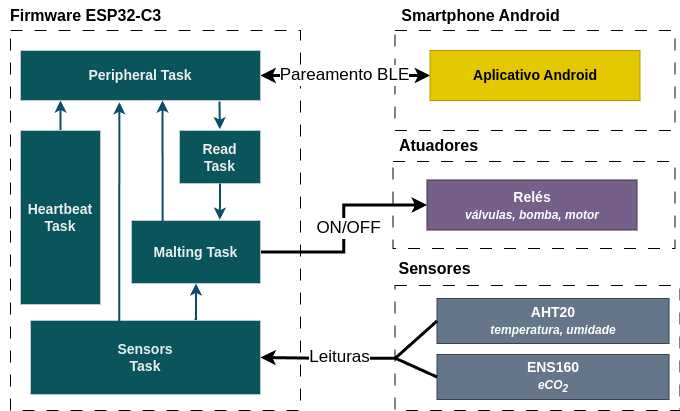
\includegraphics[width=1.0\textwidth]{TarefasAssincronas.drawio.png}

    {\centering\footnotesize Fonte: Autoria própria.\par}
\end{figure}

A tarefa \texttt{read\_task} fica aguardando o recebimento de \textit{bytes}. Quando um pacote é recebido, essa tarefa delega o tratamento dos dados para \texttt{task\_handler}, que, por sua vez, direciona os dados para outros módulos de acordo com o primeiro \textit{byte} do \textit{array} (lista). Por exemplo, ilustrado pela \autoref{fig:ReadTaskDrawio}, se o primeiro \textit{byte} for igual a 1, vai acionar o módulo de alteração dos parâmetros, que são utilizados para a realização da malteação — que é iniciada quando o \textit{array} inicia com 255.

\begin{figure}[ht]
    \centering
    \caption{Lógica do recebimento de comandos do dispositivo}
    \label{fig:ReadTaskDrawio}
    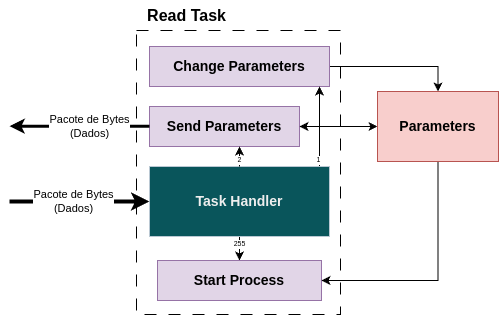
\includegraphics[width=0.7\textwidth]{ReadTask.drawio.png}

    {\centering\footnotesize Fonte: Autoria própria.\par}
\end{figure}

\subsection{Algoritmos de Controle do Processo de Malteação}
A sequência de maceração, germinação e secagem foi modelada no subdiretório \texttt{malting\_stages} em módulos especializados (\texttt{steeping.py}, \texttt{germination.py}, \texttt{kilning.py}). Cada etapa opera como uma corrotina independente, monitorando variáveis críticas com base nas condicionais dos parâmetros recebidos via Bluetooth. A estrutura assíncrona permitiu a execução não bloqueante desses processos, essencial para a continuidade da comunicação Bluetooth mesmo durante o processo. As lógicas de marcação de tempo foram desenvolvidas com o uso do módulo utilitário \texttt{uptime.py}, que se baseia no tempo total de execução do dispositivo.

\begin{figure}[ht]
    \centering
    \caption{Fluxograma do controle planejado para o algoritmo de malteação}
    \label{fig:logicamalteacao}
    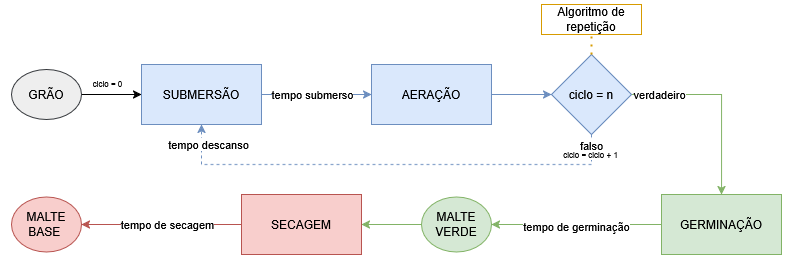
\includegraphics[width=1.0\textwidth]{logicamalteacao.png}

    {\centering\footnotesize Fonte: Autoria própria.\par}
\end{figure}

  
\section{Desenvolvimento do Aplicativo}
\subsection{Ambiente e Ferramentas de Desenvolvimento}

O ambiente de desenvolvimento foi estabelecido utilizando a IDE Android Studio (Koala Feature Drop - 2024.1.2) com linguagem Kotlin na versão 1.9.10. Os testes foram conduzidos em um dispositivo físico com Android 14, garantindo compatibilidade com as APIs mais recentes do sistema operacional. Escolheu-se o ecossistema Android Jetpack como base tecnológica devido a sua estabilidade e suporte oficial da plataforma Google para desenvolvimento de aplicativos.

\subsection{Arquitetura e Padrões de Projeto}

Adotou-se uma arquitetura em camadas conforme as diretrizes de boas práticas do Android Moderno, estruturada em três módulos principais: \textit{data}, \textit{domain} e \textit{presentation}. O módulo \textit{data} concentra a gestão de fluxos de informação, incluindo a comunicação \textit{Bluetooth} e o armazenamento local de dados, implementado com o uso das bibliotecas \textit{Room} e \textit{DataStore}. A \textit{Room} é uma biblioteca de que facilita o acesso a bancos SQLite no sistema Android \cite{android_room}. Já a \textit{DataStore} é projetada para armazenar preferências e pequenas quantidades de dados de forma mais eficiente \cite{android_datastore}.

Na camada \textit{domain}, implementou-se a lógica de negócios e o tratamento de dados. Por fim, a camada de \textit{presentation} foi construída com \textit{Jetpack Compose}, utilizando os princípios do \textit{Design Material 3} que define diretrizes de usabilidade, hierarquia visual e acessibilidade para o desenvolvimento de interfaces \cite{material3}.

\begin{figure}[ht]
    \centering
    \caption{Diagrama da arquitetura em camadas}
    \label{fig:layerarch}
    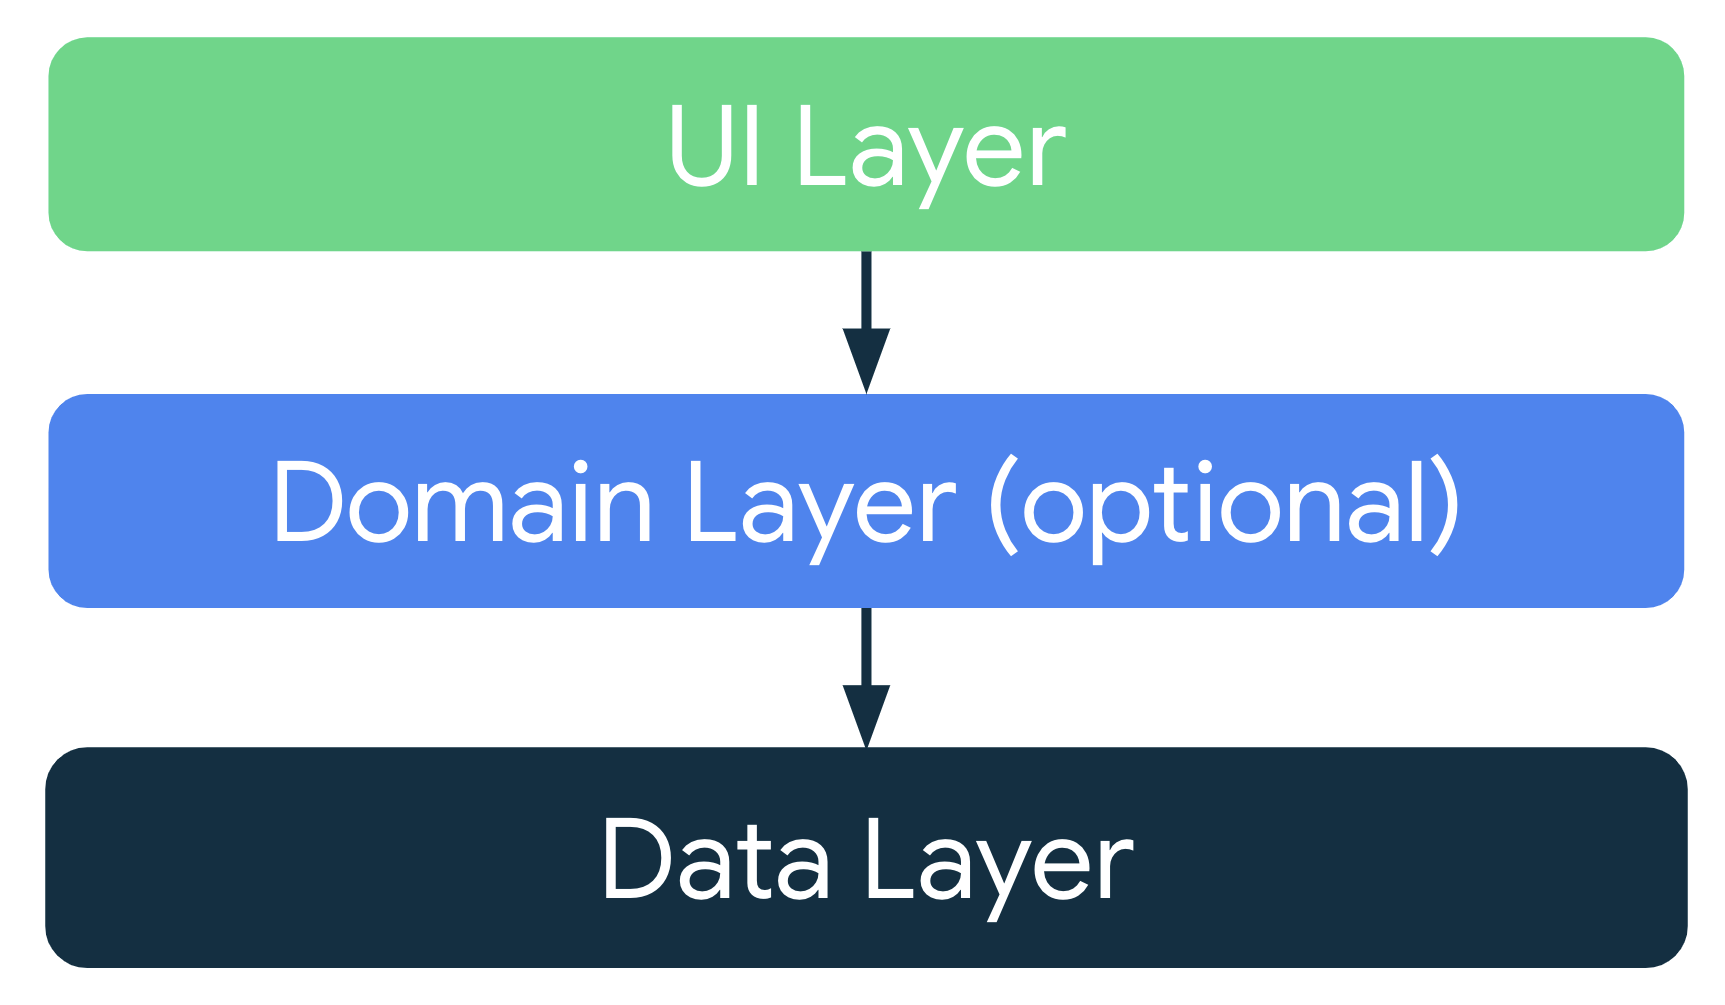
\includegraphics[width=0.6\textwidth]{layerarch.png}

    {\centering\footnotesize Fonte: Developers Android.\par}
\end{figure}

\section{Documentação}
A gestão do código foi implementada mediante a utilização do sistema de controle de versão Git, com hospedagem pública em dois repositórios GitHub dedicados: um para o firmware (acesso em: \url{https://github.com/NicolasDezan/ESP32C3-MaltingControl.git}) e outro para o aplicativo Android (acesso em: \url{https://github.com/NicolasDezan/MALT-ESP.git}). A separação em repositórios distintos buscou garantir a modularidade entre os componentes de software, além de facilitar a manutenção independente de cada projeto.

% \subsection{Tutoriais}
% Talvez eu grave tutoriais mostrando os códigos e o sistema funcionando etc etc etc
% Se sobrar tempo e se os videos ficarem legais eu vou incluir uma fala do tipo:
% A documentação técnica incluiu tutoriais em vídeo externos (links no arquivo \texttt{README.md}) detalhando processos críticos como configuração inicial do ESP32-C3 e emparelhamento Bluetooth.
  \chapter[Resultados e discussão]{Resultados e discussão}

\section{Análise do código}
\subsection{Comunicação Bluetooth}

A comunicação entre o firmware e o aplicativo é realizada por meio do BLE, a qual impõe uma limitação significativa: por padrão, cada pacote transmitido ou recebido possui um tamanho útil máximo de 20 bytes. Isso ocorre porque a MTU (\textit{Maximum Transmission Unit}) inicial, definida pela especificação Bluetooth, é de 23 bytes, sendo 3 reservados ao cabeçalho do protocolo ATT (\textit{Attribute Protocol}), restando 20 bytes para os dados \cite{ble_memfault}. Com base nisso, o código foi estruturado de forma a otimizar o uso dos pacotes disponíveis, minimizando a quantidade de transmissões necessárias e, consequentemente, aumentando a eficiência da comunicação.

Para isso, optou-se por transmitir dados diretamente no formato \texttt{byte}, o que, por consequência, permite o envio de até 20 valores distintos em um único pacote. Essa abordagem, no entanto, limita os valores possíveis ao intervalo de 0 a 255, conforme a representação padrão de um \texttt{byte}. Em situações onde foi necessário ultrapassar esse limite, foi implementada uma lógica de fragmentação dos dados, permitindo a representação de valores mais elevados por meio da combinação de dois ou mais bytes. Com esse método, tornou-se possível transmitir qualquer número, com precisão suficiente para valores decimais simples.

Essa lógica foi aplicada, por exemplo, na transmissão da informação referente ao percentual de uso da memória RAM, que exige a representação de números com casas decimais. Nessa aplicação específica, o valor percentual é multiplicado por 100 e, em seguida, dividido em dois bytes para envio, sendo reconstituído com a operação inversa no aplicativo receptor (\autoref{lst:sendheartbeat}).

\lstinputlisting[
    language=Python,
    caption=Tarefa periódica de envio de heartbeat,
    label={lst:sendheartbeat}
    ]{algoritmos/send-heartbeat-task.py}

A estratégia de triagem dos dados recebidos parte da utilização do primeiro byte do pacote como identificador, permitindo a categorização e o encaminhamento adequado de cada mensagem. Para facilitar essa operação e melhorar a legibilidade do código, foram implementadas duas classes – \texttt{ReadList} e \texttt{WriteList} – que reservam os 256 valores possíveis para identificadores (\autoref{lst:classreadlist}). Essa abordagem permite que cada valor atribuído seja mapeado a uma ação específica, otimizando o fluxo de comunicação entre o \textit{firmware} e o aplicativo.

Para exemplificar, na função \texttt{def send\_heartbeat\_task()} (\autoref{lst:sendheartbeat}), a variável \texttt{message} representa um \textit{array} construído por meio da classe \texttt{WriteList}, de onde é extraído o identificador correspondente. Este identificador é utilizado no aplicativo receptor para direcionar o tratamento da mensagem, garantindo a correta interpretação dos dados enviados.

\lstinputlisting[
    language=Python,
    caption=Definição de constantes de identifação de pacote,
    label={lst:classreadlist}
    ]{algoritmos/classreadlist.py}
  
A lógica de comunicação implementada no aplicativo Android segue o mesmo princípio de identificação adotado no firmware. O primeiro byte do pacote recebido é utilizado como identificador, sendo interpretado para direcionar o tratamento adequado dos dados (\autoref{lst:appkotlindata}). Por exemplo, quando esse identificador assume o valor 255, entende-se que o pacote refere-se ao sinal de \textit{heartbeat} enviado periodicamente pelo ESP32, contendo também o percentual de uso da memória RAM (\autoref{lst:condicionaldereceberusodememoria}).

\lstinputlisting[
    language=Python,
    caption=Seção de triagem dos dados recebidos (aplicativo),
    label={lst:appkotlindata}
    ]{algoritmos/data-handling.kt}

\lstinputlisting[
    language=Python,
    caption=Tratamento do pacote identificado com '255',
    label={lst:condicionaldereceberusodememoria}
    ]{algoritmos/condicionaldereceberusodememoria.kt}

Nesse contexto, o aplicativo interpreta os bytes seguintes como valores numéricos que representam, respectivamente, a parte inteira e a parte decimal da porcentagem. Esses valores são somados após a conversão para o formato numérico adequado, resultando em um valor final com duas casas decimais (\autoref{lst:condicionaldereceberusodememoria}). Esse número é então utilizado para atualizar a interface do usuário com a informação atualizada sobre o consumo de memória do dispositivo.

Além da extração dos dados de uso de memória, o recebimento do identificador 255 também aciona uma função interna responsável por sinalizar a chegada do \textit{heartbeat}. Esse mecanismo funciona como um pulso periódico enviado pelo firmware, cuja função principal é indicar que o dispositivo segue ativo e em comunicação com o aplicativo. No aplicativo, esse pulso ativa um recurso visual na interface: uma indicação em forma de círculo que pisca a cada novo recebimento. Esse indicador atua como um monitor de conexão em tempo real, permitindo ao usuário verificar de forma intuitiva se a comunicação Bluetooth está estável. Caso o pulso deixe de ser recebido por um intervalo prolongado, o usuário deve observar que ocorreu a perda de sinal ou falha de comunicação, evitando a falsa impressão de que o sistema permanece operacional quando, na verdade, pode estar congelado ou desconectado.

Esse modelo de tratamento baseado em identificadores garante clareza na separação das funções e facilita futuras expansões, mantendo o código modular e de fácil manutenção.


\subsection{Parâmetros de malteação}

Os parâmetros de malteação correspondem às variáveis de controle utilizadas para configurar e ajustar o processo, como tempos de etapa, temperatura alvo e outros valores relevantes. Esses dados são essenciais para garantir a execução correta das etapas automatizadas.

Durante a inicialização do sistema, o firmware realiza a leitura de um arquivo de configuração persistente, armazenado localmente na memória do ESP32. Esse arquivo, no formato JSON, contém os valores salvos da última configuração utilizada. O conteúdo lido é mapeado internamente para as variáveis de controle do sistema, tornando-as acessíveis para os demais módulos do firmware.

Além da leitura, o sistema também permite a atualização desses parâmetros via comunicação Bluetooth. Sempre que o aplicativo envia novos valores, eles são armazenados temporariamente, validados e, posteriormente, gravados no arquivo de configuração. Isso garante que as alterações permaneçam ativas mesmo após desligamentos ou reinicializações.

A lógica geral de carregamento e persistência dos parâmetros é representada na \autoref{fig:fluxoparametros}, que ilustra o fluxo completo de inicialização e atualização dos dados operacionais do malteador.

\begin{figure}[ht]
    \centering
    \caption{Fluxo de inicialização e atualização dos parâmetros de malteação.}
    \label{fig:fluxoparametros}
    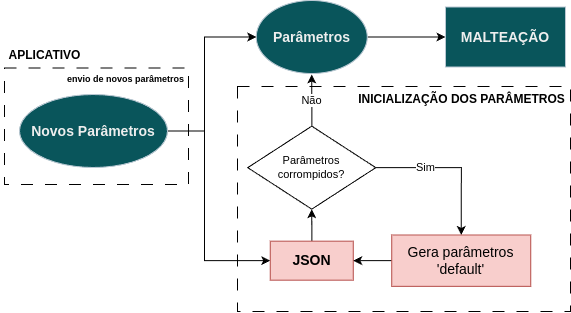
\includegraphics[width=0.9\textwidth]{fluxoparametros.png}

    {\centering\footnotesize Fonte: Autoria própria.\par}
\end{figure}

Os parâmetros de malteação foram otimizados para que seus valores pudessem ser representados dentro da faixa de um único byte, permitindo até 256 variações distintas por parâmetro. Essa decisão buscou equilibrar a precisão necessária para o controle do processo com a eficiência na comunicação via Bluetooth, já que o envio de todos os parâmetros em um único pacote reduz o tempo de transmissão e minimiza o risco de perda de pacotes.

Embora essa abordagem limite a resolução de cada parâmetro, ela se mostra adequada frente às grandezas envolvidas no processo. Caso, em futuras otimizações, identifique-se a necessidade de representar valores com maior precisão, a arquitetura atual do sistema permite a adição de bytes extras sem impactos significativos na estrutura dos módulos.

A conversão dos valores numéricos para um único byte é feita por meio de uma transformação linear, na qual o valor transmitido (inteiro entre 0 e 255) é multiplicado por um fator de escala e somado a um valor mínimo admissível. Esse procedimento garante que a representação final esteja sempre dentro da faixa operacional válida para cada variável.

As Tabelas~\ref{tab:coefmac}, \ref{tab:coefgerm} e \ref{tab:coefsec} apresentam os coeficientes utilizados para a reconstrução dos valores reais a partir dos dados recebidos via Bluetooth. Para cada parâmetro, aplica-se a seguinte fórmula:

\begin{center}
    \textit{valor real} = (\textit{byte recebido} × MULT\_TEN) + MIN\_VALUE
\end{center}

Esse mesmo modelo é utilizado na conversão inversa, durante a serialização dos dados antes da transmissão, garantindo consistência entre os módulos do firmware e do aplicativo.

\begin{table}[ht]
    \caption{Coeficientes de reconstrução — Etapa de Maceração}
    \label{tab:coefmac}
    \centering
    \begin{tabular}{lcc}
        \hline
        \bfseries Parâmetro & \bfseries MULT\_TEN & \bfseries MIN\_VALUE \\
        \hline
        Tempo Submerso     & 1.0  & 1.0   \\
        Volume de Água     & 10.0 & 200.0 \\
        Tempo de Descanso  & 0.1  & 0.0   \\
        Número de Ciclos   & 1.0  & 1.0   \\
        \hline
    \end{tabular}
    
    {\centering\footnotesize Fonte: Autoria própria.\par}
\end{table}

\begin{table}[ht]
    \caption{Coeficientes de reconstrução — Etapa de Germinação}
    \label{tab:coefgerm}
    \centering
    \begin{tabular}{lcc}
        \hline
        \bfseries Parâmetro & \bfseries MULT\_TEN & \bfseries MIN\_VALUE \\
        \hline
        Nível de Rotação    & 1.0 & 0.0  \\
        Tempo Total         & 1.0 & 24.0 \\
        Volume de Água      & 1.0 & 100.0 \\
        Adição de Água      & 1.0 & 10.0 \\
        \hline
    \end{tabular}
    
    {\centering\footnotesize Fonte: Autoria própria.\par}
\end{table}

\begin{table}[ht]
    \caption{Coeficientes de reconstrução — Etapa de Secagem}
    \label{tab:coefsec}
    \centering
    \begin{tabular}{lcc}
        \hline
        \bfseries Parâmetro & \bfseries MULT\_TEN & \bfseries MIN\_VALUE \\
        \hline
        Temperatura  & 1.0 & 40.0 \\
        Tempo Total  & 0.1 & 1.0  \\
        \hline
    \end{tabular}
    
    {\centering\footnotesize Fonte: Autoria própria.\par}
\end{table}

Na \autoref{tab:parametros}, são listados todos os parâmetros disponíveis no sistema, acompanhados de suas respectivas faixas de valores operacionais, definidas conforme os limites estabelecidos.

\begin{table}[ht]
    \caption{Faixa de valores possíveis para cada parâmetro.}
    \label{tab:parametros}
    \centering
    \begin{tabular}{cccc}
        \hline
        \bfseries Parâmetro & \bfseries Etapa & \bfseries Faixa de Valores & \bfseries Unidade \\
        \hline
        Tempo Submerso & Maceração & 1 -- 256  & horas \\
        Volume de Água & Maceração & 200 -- 2750 & mL \\
        Tempo de Descanso & Maceração & 0.0 -- 25,5 & horas \\
        Número de Ciclos & Maceração & 1 -- 256 & ciclos \\
        Nível de Rotação & Germinação & 0 -- 255 & -- \\
        Tempo Total & Germinação & 24 -- 279 & horas \\
        Volume de Água & Germinação & 100 -- 355 & mL \\
        Adição de Água & Germinação & 10 -- 265 & minutos \\
        Temperatura & Secagem & 40 -- 295 & $^{\circ}$C \\
        Tempo Total & Secagem & 1.0 -- 26.5 & horas \\
        \hline
    \end{tabular}

    {\centering\footnotesize Fonte: Autoria própria.\par}
\end{table}



\subsection{Algoritmo da malteação}

O controle automatizado da malteação foi implementado com base em uma lógica assíncrona, permitindo a execução simultânea de múltiplas tarefas relacionadas ao processo. A arquitetura do algoritmo principal é centrada em um sistema de estados, no qual cada etapa do processo (maceração, germinação e secagem) é tratada como um estágio independente, com mecanismos de inicialização, monitoramento e interrupção.

A execução do processo é iniciada a partir de um comando enviado pelo aplicativo, o que ativa a função responsável pela coordenação da malteação. Essa função inicializa o estado global e delega a execução para funções específicas de cada etapa, que operam com base nas configurações previamente definidas (parâmetros).

Durante toda a execução, o sistema monitora constantemente um sinal de interrupção, que pode ser acionado a qualquer momento via comunicação Bluetooth. Essa lógica garante que o processo possa ser encerrado de forma segura e imediata, sem comprometer a integridade das etapas já concluídas.

\subsubsection{Maceração}

A etapa de maceração é composta por dois fluxos assíncronos que atuam de forma paralela: o controle térmico, responsável por manter a temperatura adequada do sistema, e o controle de tempo, que regula a execução dos ciclos de hidratação.

Cada ciclo da maceração é formado por quatro subetapas executadas sequencialmente:

\begin{enumerate}
    \item \textbf{Enchimento}: o reservatório é preenchido com água até o volume desejado.
    \item \textbf{Imersão}: os grãos permanecem submersos pelo tempo programado.
    \item \textbf{Drenagem}: a água é escoada do sistema.
    \item \textbf{Repouso}: há uma pausa antes do próximo ciclo.
\end{enumerate}

Essas fases são repetidas conforme o número de ciclos configurado pelo usuário. A execução da etapa de maceração pode ser representada de forma resumida na Tabela~\ref{tab:maceracao-fluxo}.

\begin{table}[ht]
    \caption{Fluxo de controle da etapa de maceração}
    \label{tab:maceracao-fluxo}
    \centering
    \begin{tabular}{>{\bfseries}c p{10cm}}
        \hline
        Fase & Descrição \\
        \hline
        Inicialização & Define o estado do sistema como \texttt{steeping}, carrega os parâmetros de ciclo e inicia tarefas assíncronas. \\
        Controle térmico & Mantém a temperatura dentro do intervalo alvo por meio de resfriamento ativo. Executado em paralelo. \\
        Controle de tempo & Executa a sequência de subetapas (enchimento, imersão, drenagem, repouso) para cada ciclo. \\
        Interrupção & A cada subetapa, o sistema verifica continuamente se houve solicitação de parada. \\
        Finalização & Ao término dos ciclos ou interrupção, o sistema atualiza o estado para inativo. \\
        \hline
    \end{tabular}
    
    {\centering\footnotesize Fonte: Autoria própria.\par}
\end{table}

O controle de válvulas, tanto para enchimento quanto para drenagem, segue um modelo baseado no tempo de abertura, adicionando o volume necessário para a operação. Apesar de simplificado, esse método pode ser ajustado posteriormente com base em calibrações que relacionem diretamente o tempo de válvula aberta ao volume de água processado. Esse aspecto é fundamental para permitir futuras melhorias sem a necessidade de reescrita da estrutura de controle.

A lógica de controle de temperatura foi implementada como uma tarefa paralela, executada em segundo plano com checagens periódicas e resposta imediata ao sinal de interrupção. Embora o protótipo atual ainda não possua capacidade física de controle térmico ativo (resfriamento), essa tarefa já está incorporada de forma modular no firmware, permitindo que sensores e atuadores possam ser integrados futuramente sem necessidade de grandes modificações estruturais. Essa abordagem garante escalabilidade e separação de responsabilidades, mantendo a coesão da arquitetura.

Ao final da execução dos ciclos de maceração, o sistema redefine o estado da etapa como inativo e passa automaticamente para o próximo estágio do processo, aguardando o início da germinação.

\subsubsection{Germinação}

A etapa de germinação (\textit{germination}) mantém a estrutura introduzida na maceração, com múltiplas tarefas assíncronas atuando de forma coordenada. Ao entrar nesse estágio, o sistema atualiza o estado global e ativa quatro tarefas principais, que operam em paralelo:

\begin{itemize}
    \item \textbf{Controle de tempo}: cronômetro responsável por definir a duração total da germinação.
    \item \textbf{Controle de temperatura}: ajusta ou monitora a temperatura ambiente.
    \item \textbf{Controle de umidade}: umidifica os grãos periodicamente.
    \item \textbf{Controle de rotação}: ativa mecanismos de movimentação dos grãos para arejamento.
\end{itemize}

Essas tarefas compartilham uma variável de sinalização comum, que permite a interrupção imediata da etapa caso o processo seja cancelado via aplicativo. A Tabela~\ref{tab:germinacao_fluxo} resume a lógica operacional da etapa de germinação.

\begin{table}[ht]
    \caption{Fluxo de controle da etapa de germinação.}
    \label{tab:germinacao_fluxo}
    \centering
    \begin{tabular}{>{\bfseries}c p{10cm}}
        \hline
        Fase & Descrição \\
        \hline
        Inicialização & Atualiza o estado global para \texttt{germination} e carrega os parâmetros definidos. \\
        Controle temporal & Inicia o cronômetro principal da etapa. Ao fim do tempo total, sinaliza término da germinação. \\
        Controle ambiental & Controla e monitora temperatura e umidade em paralelo ao tempo. \\
        Controle de rotação & Aciona o sistema de movimentação dos grãos em intervalos regulares. \\
        Interrupção & Todas as tarefas verificam sinal de parada a cada ciclo. \\
        Finalização & Ao término do tempo ou interrupção, o sistema limpa o estado e prepara a etapa seguinte. \\
        \hline
    \end{tabular}

    {\centering\footnotesize Fonte: Autoria própria.\par}
\end{table}

A umidificação periódica dos grãos é feita por meio de ciclos adicionam de água. O algoritmo alterna entre a abertura de válvulas para umidificar o ambiente e pausas programadas para não encharcar os grãos. Essa tarefa permanece ativa enquanto o estágio estiver em execução, repetindo os ciclos conforme o necessário. O controle de temperatura segue o mesmo princípio adotado na etapa anterior, sendo executado como tarefa independente que verifica periodicamente o estado do sistema, permitindo ajustes térmicos futuros.

O reservatório de água do protótipo foi planejado para suportar 5 litros, estima-se que este valor seja suficiente para o processo. Apesar disso, caso seja necessário, a implementação de um sensor de distância ultrassom para acompanhamento do nível do tanque será simples dada a arquitetura do firmware. 

Além disso, durante a germinação, o sistema realiza rotações constantes, para o revolvimento dos grãos com o objetivo de garantir a aeração e evitar o emaranhamento das radículas. Existe, também, leituras de CO$_{2}$ durante essa etapa para que seja possível emitir um alerta para o operador caso se atinja valores prejudiciais ao crescimento dos grãos.

\subsubsection{Secagem}

Encerrada a germinação, inicia-se a última etapa do processo: a secagem (\textit{kilning}). Nesta fase, o objetivo é reduzir a umidade dos grãos e interromper a atividade enzimática, preservando as características desejadas do malte. A lógica geral mantém o padrão assíncrono das etapas anteriores, com três tarefas paralelas operando de forma coordenada: controle de tempo, temperatura e rotação.

A Tabela~\ref{tab:secagem_fluxo} detalha o fluxo operacional da etapa de secagem:

\begin{table}[ht]
    \caption{Fluxo de controle da etapa de secagem}
    \label{tab:secagem_fluxo}
    \centering
    \begin{tabular}{>{\bfseries}c p{10cm}}
        \hline
        Fase & Descrição \\
        \hline
        Inicialização & Atualiza o estado global para \texttt{kilning} \\
        Controle temporal & Gerencia a duração total do estágio através de contagem regressiva baseada nos parâmetros \\
        Controle térmico & Mantém temperatura elevada, utilizando ciclos de aquecimento e monitoramento contínuo \\
        Controle de rotação & Ativa mecanismos de revolvimento em intervalos programados para homogeneização \\
        Interrupção & Verificação contínua de sinal de parada durante todas as subetapas \\
        Finalização & Desativa sistemas térmicos e mecânicos, atualiza estado para inativo \\
        \hline
    \end{tabular}

    {\centering\footnotesize Fonte: Autoria própria.\par}
\end{table}

O controle de tempo define a duração total do estágio, monitorando continuamente a contagem regressiva com base nos parâmetros definidos pelo usuário. Já a temperatura, nesse estágio, assume papel ainda mais crítico, visto que a secagem envolve temperaturas elevadas e potencialmente danosas ao produto se não forem adequadamente controladas.

Por fim, o controle de rotação continua presente, com o intuito de garantir a homogeneidade da secagem e evitar a formação de zonas com retenção de umidade. Essa movimentação periódica dos grãos deve assegurar uma secagem eficiente e uniforme.

A estrutura assíncrona aplicada em todas as etapas da malteação permite ao sistema operar com múltiplos controles simultâneos, com segurança, responsividade e flexibilidade. A separação lógica das funções facilita tanto a manutenção do código quanto a sua expansão, criando uma base para futuras implementações automatizadas, como a inclusão de um programa de torra.
 
\subsection{Sensores e Atuadores}

Nesta implementação, foram utilizados dois sensores, ambos com arquitetura baseada no protocolo I\textsuperscript{2}C responsáveis pela aquisição de dados para o processo:

\begin{table}[ht]
    \caption{Especificação dos sensores}
    \label{tab:sensores_atuadores}
    \centering
    \begin{tabular}{llp{8cm}}
        \hline
        \textbf{Sensor} & \textbf{Parâmetros} & \textbf{Função no processo} \\
        \hline
        AHT20 & Temperatura e umidade relativa & Monitoramento contínuo das condições ambientais durante todas as etapas da malteação \\
        ENS160 & eCO\textsubscript{2} (equivalente de CO\textsubscript{2}) & Detecção e monitoramento da atividade metabólica dos grãos na fase de germinação \\
        \hline
    \end{tabular}
    
    {\centering\footnotesize Fonte: Autoria própria.\par}
\end{table}

A leitura dos sensores ocorre de maneira contínua e assíncrona na tarefa \texttt{sensors\_task}, garantindo atualização constante dos dados. Após cada leitura, os valores de temperatura, umidade e eCO\textsubscript{2} são armazenados em variáveis globais, facilitando o acesso por outras tarefas do sistema. Para fins de transmissão Bluetooth, os valores são convertidos em bytes e enviados periodicamente para o aplicativo dentro dessa própria função.

O tratamento de falhas também foi considerado: caso a leitura de qualquer sensor falhe, o sistema atribui valor zero como padrão, garantindo que o fluxo da comunicação continue sem interrupções.

Em paralelo à leitura de sensores, o sistema também gerencia cinco atuadores principais: duas válvulas (entrada e saída de água), um motor de rotação, uma resistência térmica e uma bomba de ar. A lógica de controle desses dispositivos é encapsulada na classe \texttt{Actuator} (\autoref{lst:actuator}), desenvolvida para simplificar a manipulação dos pinos GPIO e abstrair as diferenças de lógica de acionamento.

\lstinputlisting[
    language=Python,
    caption=Classe Actuator - MicroPython,
    label={lst:actuator}
    ]{algoritmos/actuator.py} 

Cada atuador é instanciado em \texttt{actuators} com seu respectivo nome e número de pino, e armazenado em um dicionário global para facilitar o acesso dinâmico por outras partes do sistema. A classe (\autoref{lst:actuator}) disponibiliza métodos como \texttt{on()}, \texttt{off()} e \texttt{toggle()}, além de uma função de verificação de estado atual. Dessa forma, o acionamento de cada dispositivo torna-se simples, confiável e rastreável (via terminal).

Além do controle direto, foi implementada uma função de envio do estado atual dos atuadores via Bluetooth, permitindo que o aplicativo visualize, em tempo real, quais dispositivos estão ativos no momento.

\section{Aplicativo Android}\label{sec:aplicativo-android}

\subsection{Tela Inicial: Conexão}\label{subsec:conexao}
Ao inicializar o aplicativo, o usuário é direcionado à interface de conexão. Nesta tela, é exibido centralmente o status "Não conectado", acompanhado de um indicador de estado pulsante no canto superior direito, que alterna entre azul e cinza a cada segundo, quando conectado. A conexão com o dispositivo ESP32, previamente pareado via Bluetooth, é estabelecida mediante acionamento do botão "Conectar", conforme ilustrado na \autoref{fig:int-inicial}.

\begin{figure}[ht]
    \caption{Interface inicial do aplicativo.}
    \label{fig:int-inicial}
    \centering
    \subfloat[Desconectado\label{fig:first-off}]{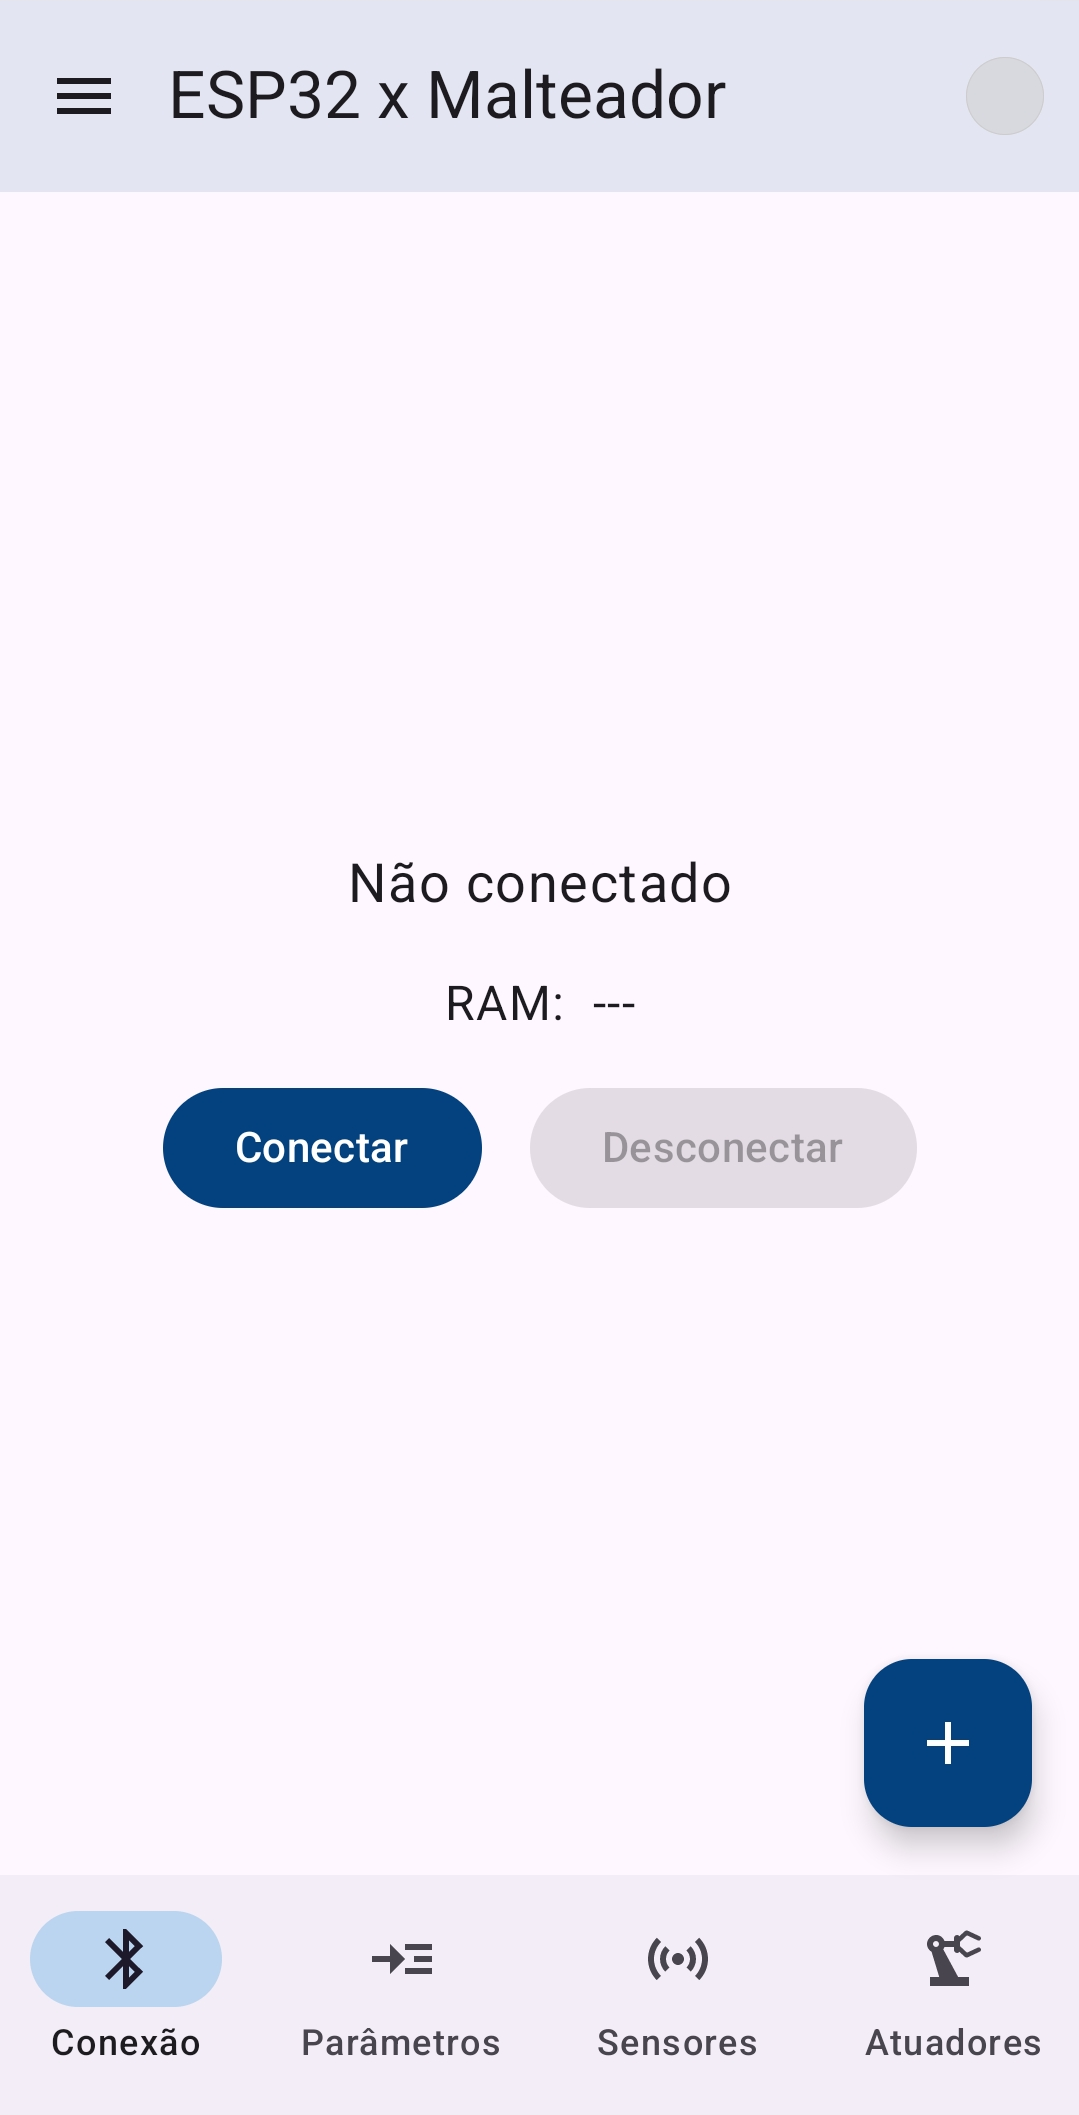
\includegraphics[width=0.3\textwidth]{first-off.png}}
    \hfill
    \subfloat[Conectado\label{fig:first-on}]{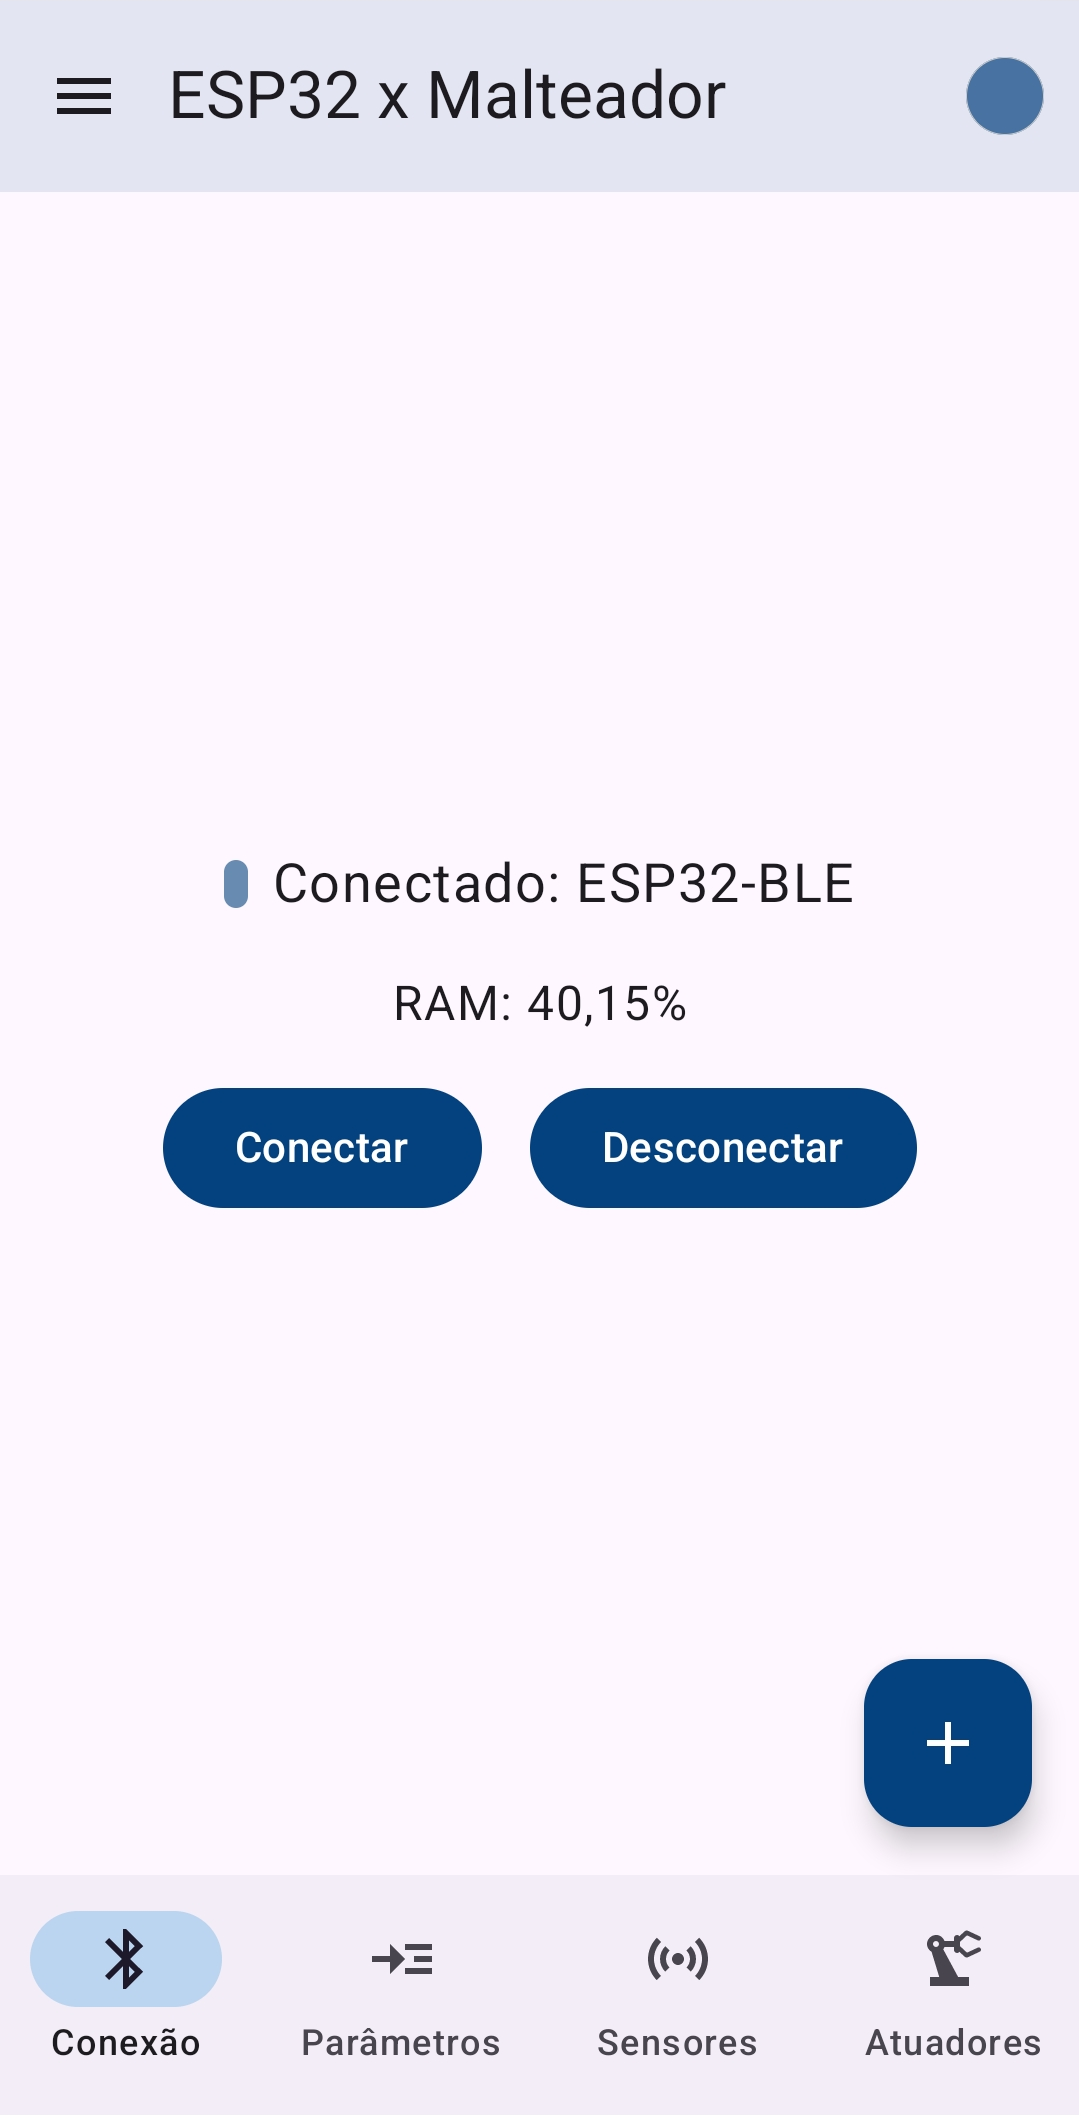
\includegraphics[width=0.3\textwidth]{first-on.png}}
    \hfill
    \subfloat[Tema escuro\label{fig:first-dark-theme}]{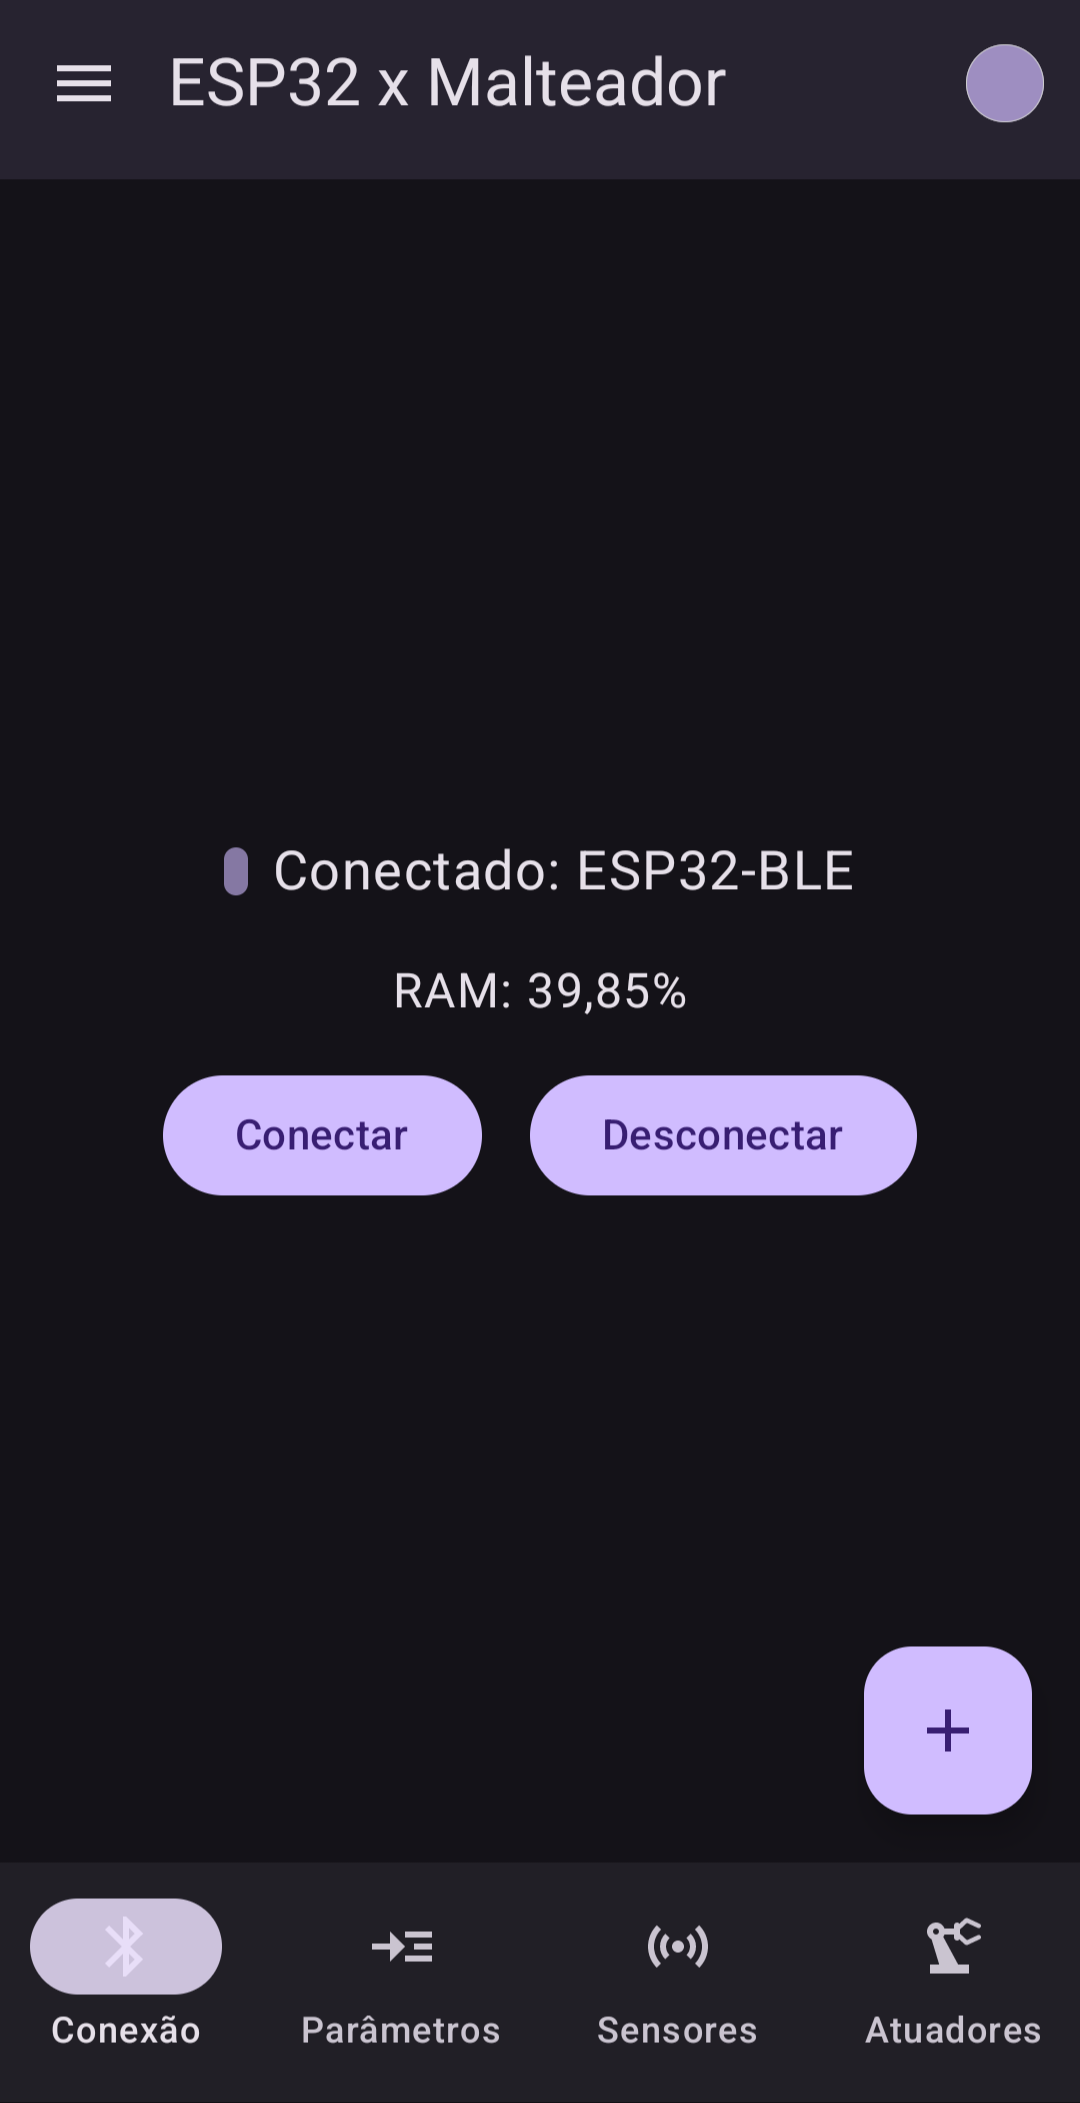
\includegraphics[width=0.3\textwidth]{first-dark-theme.png}}

    {\centering\footnotesize Fonte: Autoria própria.\par}

  \end{figure}


Ainda, na estrutura geral do \textit{Scaffold} (layout do aplicativo), destaca-se o \textit{FloatingActionButton} (FAB) no canto inferior direito. Este componente, ao ser acionado, expande um menu com funcionalidades essenciais, incluindo:

\begin{itemize}
    \item \textit{Verificar Parâmetros}, para sincronização dos parâmetros com o ESP32;
    \item \textit{Carregar Receita}, para autopreencher os parâmetros no aplicativo;
    \item \textit{Iniciar}, para enviar os parâmetros e iniciar o processo de malteação.
\end{itemize}

No canto superior esquerdo, o botão de navegação proporciona acesso ao \textit{Drawer}, um painel lateral com duas opções: "Início" (retorno à tela principal) e "Configurações" (\autoref{fig:drawer}). A tela de configurações, em sua versão atual, permite a alternância entre temas claro e escuro (\autoref{fig:int-inicial}), com previsão de expansão para personalizações avançadas, como definição de nomes de dispositivos e ajustes dos valores de UUID Bluetooth.

\begin{figure}[ht]
    \caption{Drawer do aplicativo.}
    \label{fig:drawer}
    \centering
    \subfloat[Botão de acesso ao drawer\label{fig:DrawerButton}]{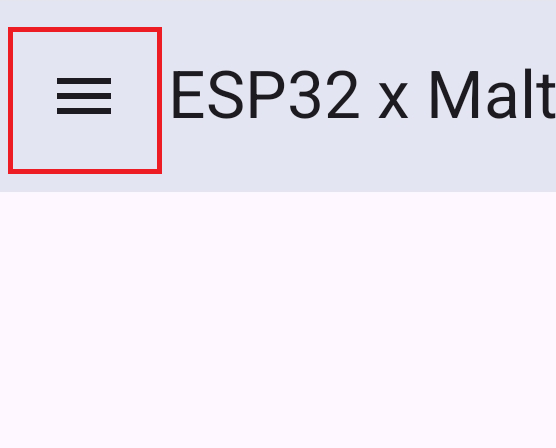
\includegraphics[width=0.3\textwidth]{DrawerButton.png}}
    \hfill
    \subfloat[Drawer aberto\label{fig:open-drawer}]{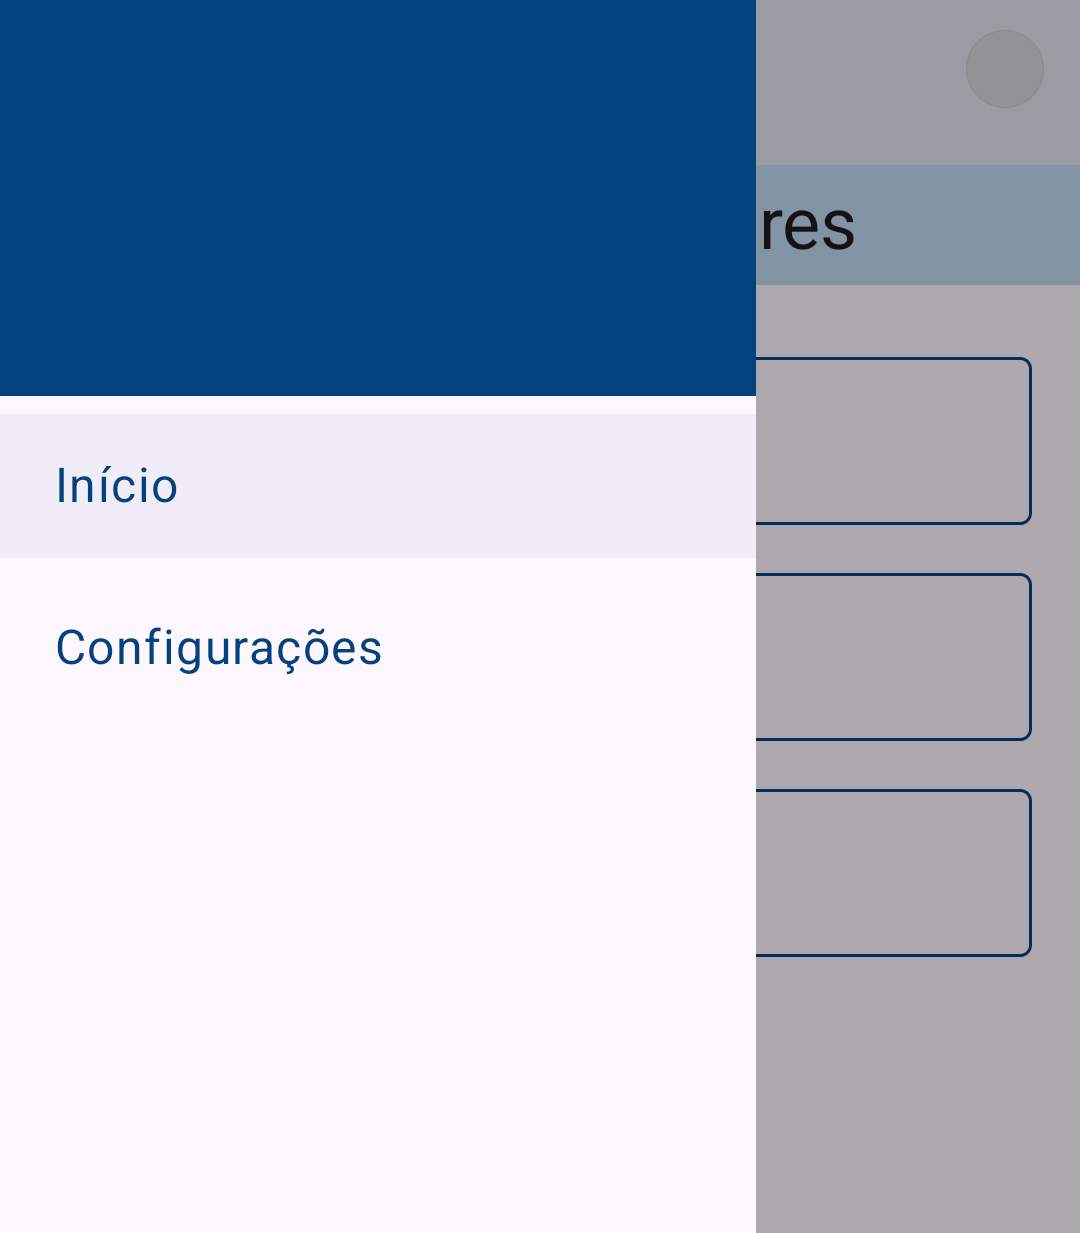
\includegraphics[width=0.3\textwidth]{open-drawer.png}}
    \hfill
    \subfloat[Tela de configurações acessada pelo drawer\label{fig:config-screen}]{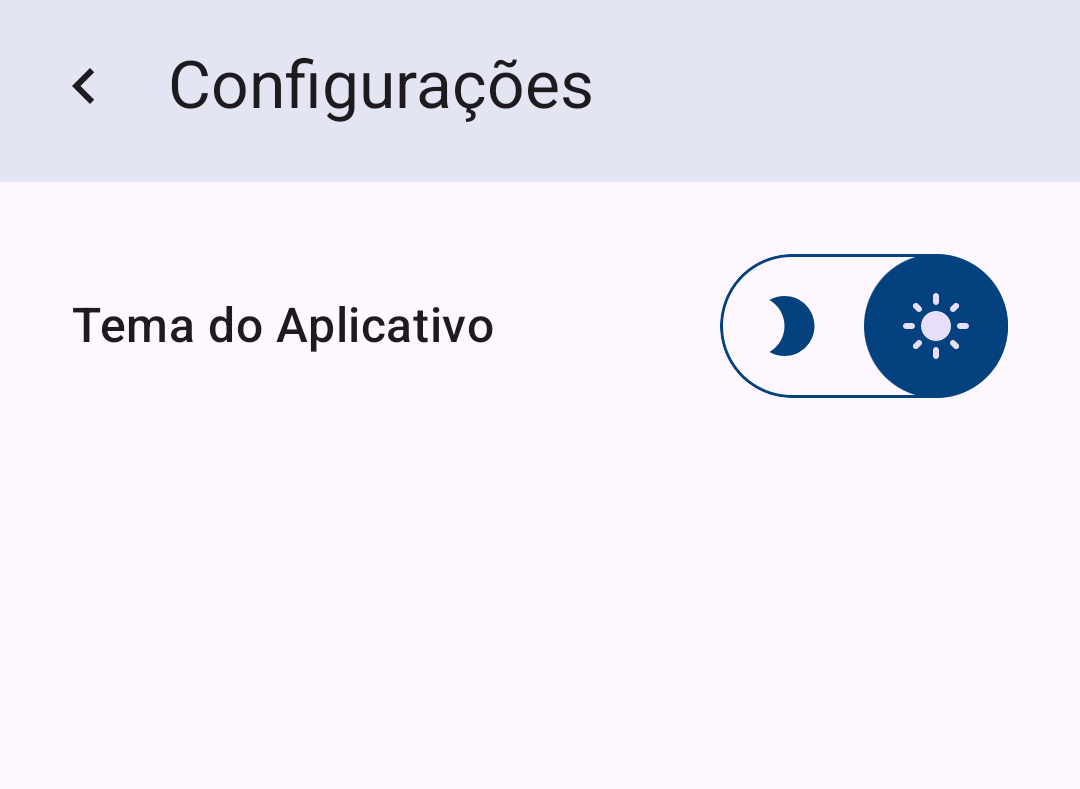
\includegraphics[width=0.3\textwidth]{config-screen.png}}

    {\centering\footnotesize Fonte: Autoria própria.\par}

  \end{figure}

\subsection{Tela de Parâmetros}\label{subsec:parametros}
A interface de parâmetros opera em dois modos distintos, conforme o estado de conexão. No modo desconectado (\autoref{fig:par-off}), os campos de entrada permanecem inativos. Quando conectado, os campos assumem codificação cromática dinâmica: tonalidade amarela para indicar valores não sincronizados ou nulos, e azul para valores válidos sincronizados com o ESP32 (\autoref{fig:parameters-state}). Valores fora da faixa operacional (\autoref{{tab:parametros}}) ou inconsistentes geram feedback visual impedindo o envio (\autoref{fig:parameters-state}), previnindo possíveis erros de extrapolação dos bytes na comunicação Bluetooth.

\begin{figure}[ht]
    \centering
    \caption{Tela de parâmetros em modo desconectado com campos inativos.}
    \label{fig:par-off}
    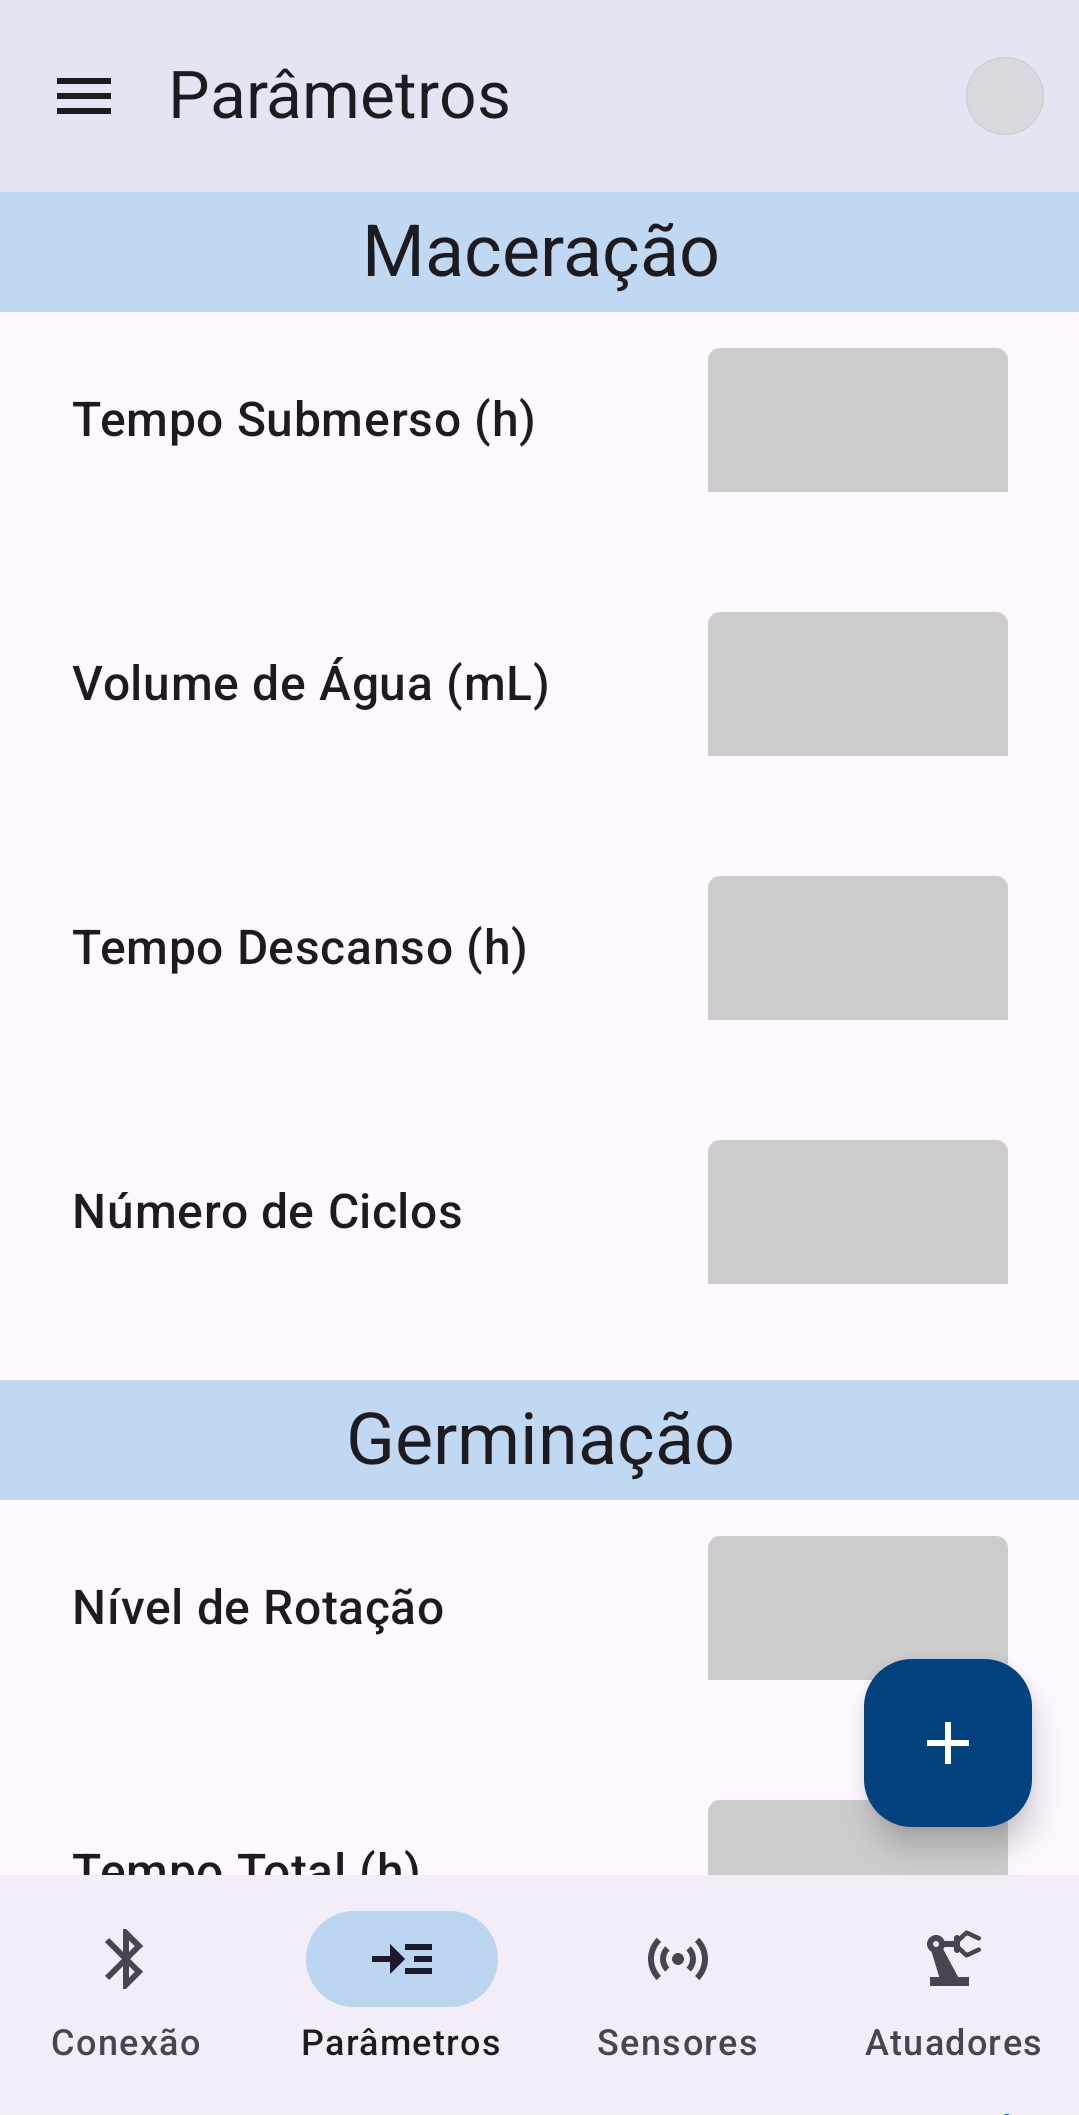
\includegraphics[width=0.32\textwidth]{par-off.png}

    {\centering\footnotesize Fonte: Autoria própria.\par}
\end{figure}

\begin{figure}[ht]
    \caption{Estados dos campos de parâmetros.}
    \label{fig:parameters-state}
    \centering
    \subfloat[Campos de parâmetros em estado não sincronizado\label{fig:input-on-yellow}]{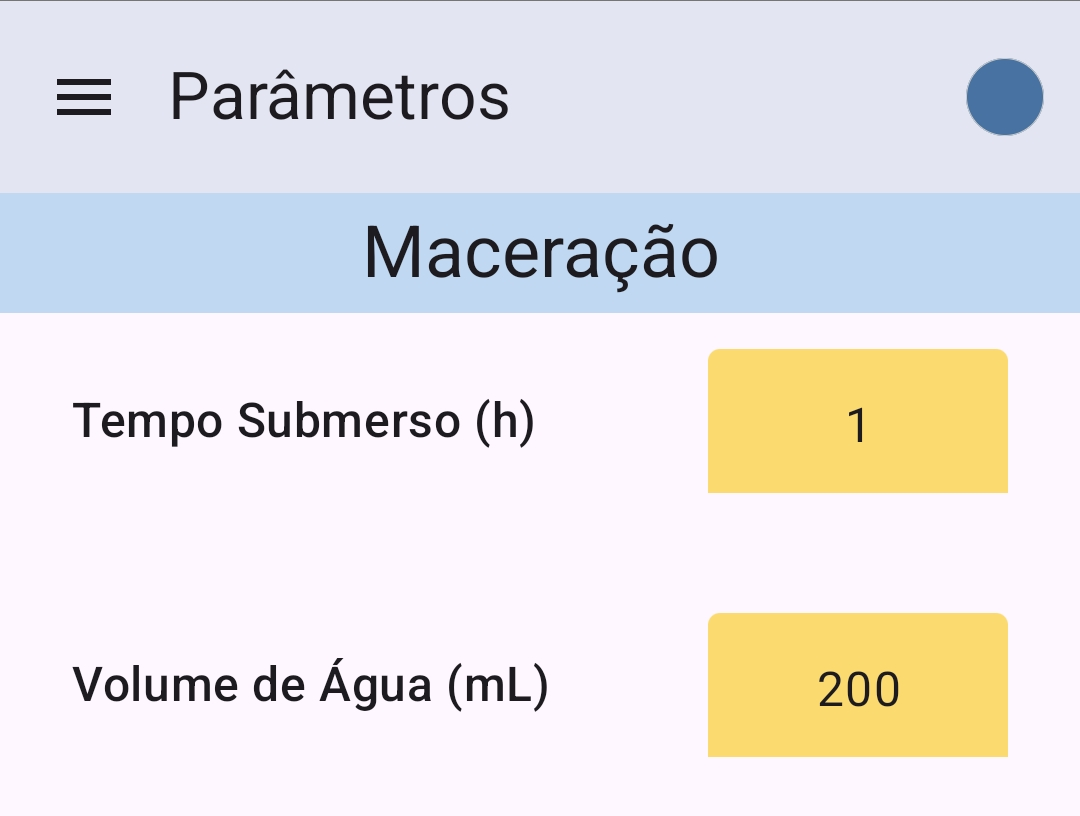
\includegraphics[width=0.4\textwidth]{input-on-yellow.png}}
    \hfill
    \subfloat[Campos de parâmetros válidos sincronizados\label{fig:input-on-blue}]{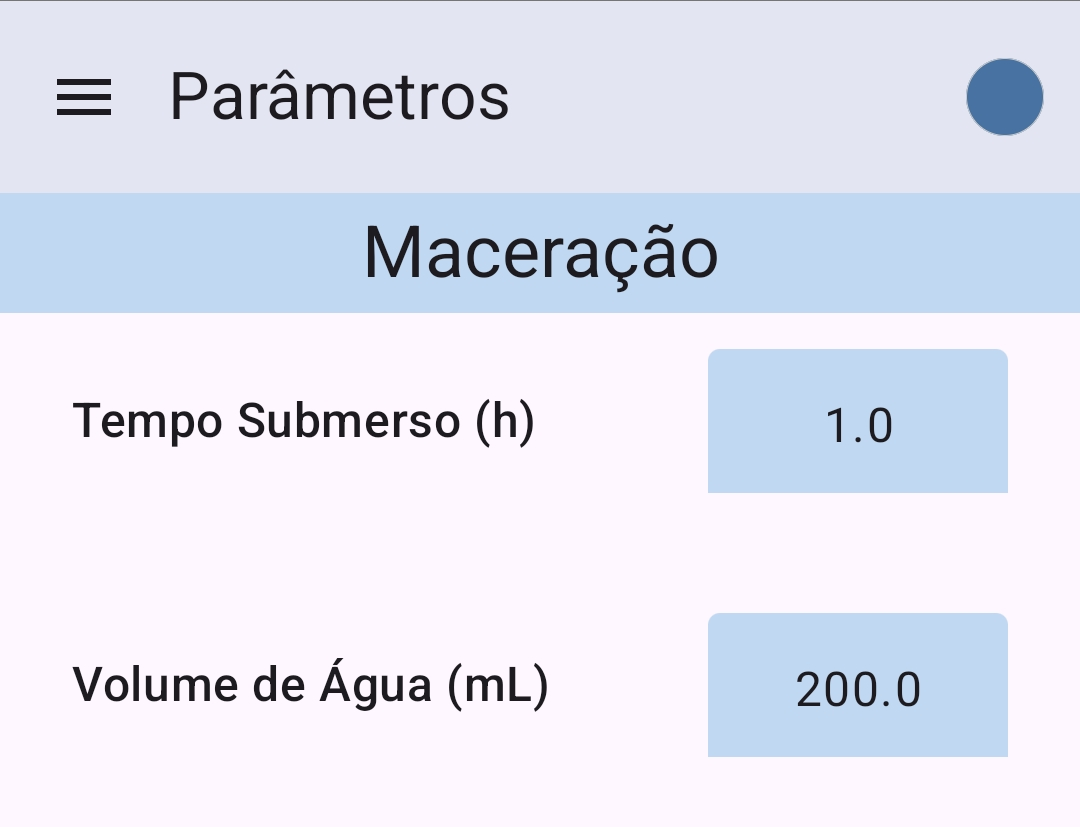
\includegraphics[width=0.4\textwidth]{input-on-blue.png}}
    \hfill
    \subfloat[Feedback visual para valores fora da faixa operacional\label{fig:out-range}]{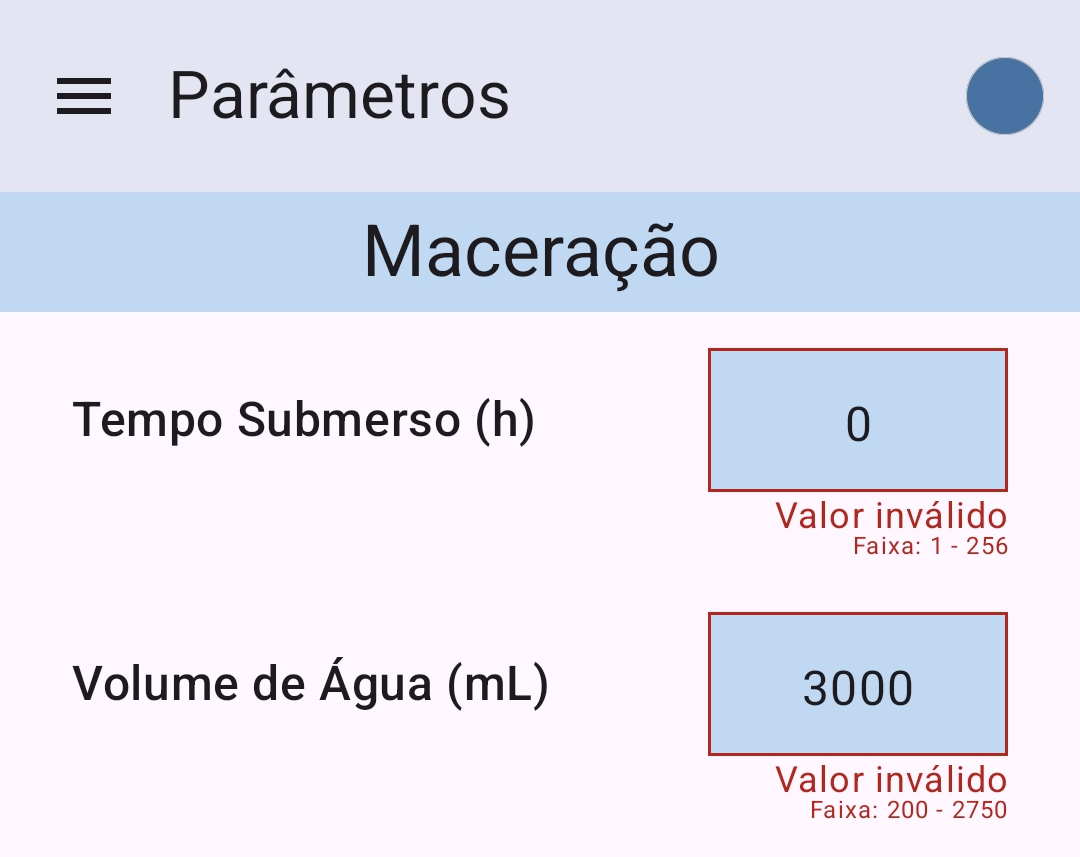
\includegraphics[width=0.4\textwidth]{out-range.png}}
    \hfill
    \subfloat[Feedback visual para valores nulos\label{fig:null-value}]{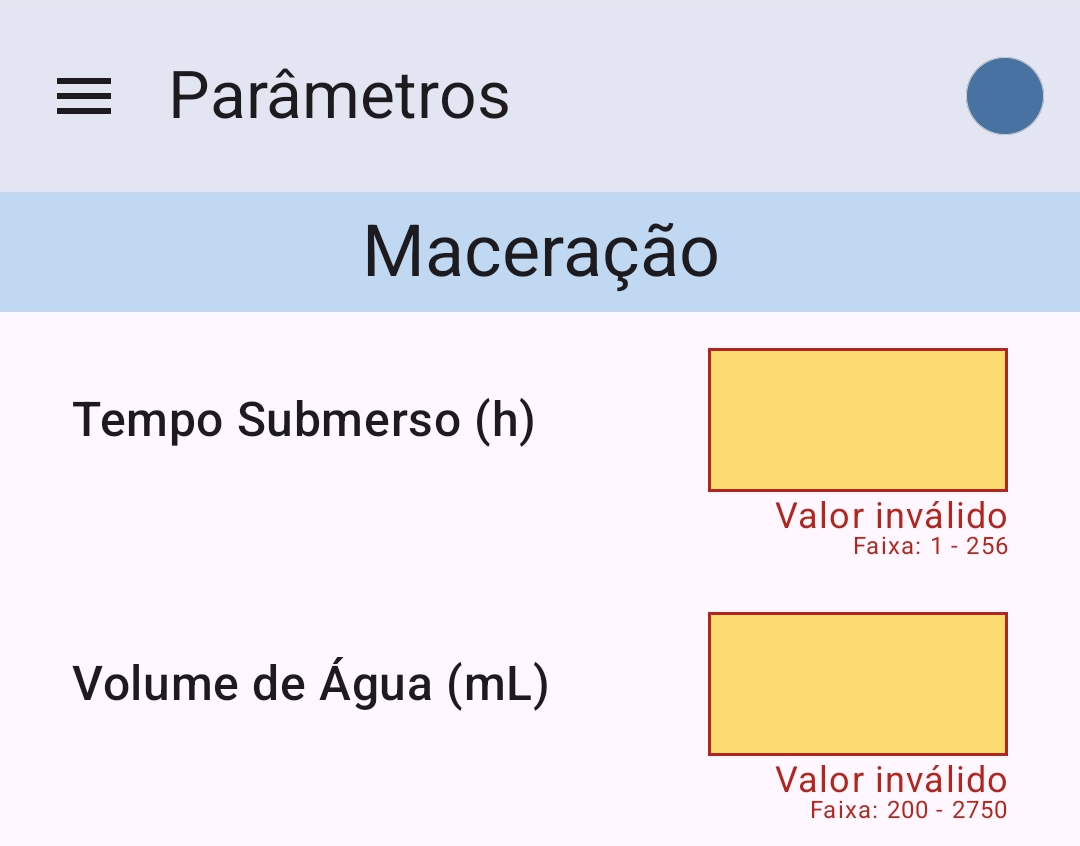
\includegraphics[width=0.4\textwidth]{null-value.png}}
    \hfill

    {\centering\footnotesize Fonte: Autoria própria.\par}

  \end{figure}


Para melhor experiência do usuário/operador, o sistema permite o armazenamento das configurações atuais de parâmetros como perfis personalizados ("receitas"), mediante nomeação em diálogo dedicado (\autoref{fig:select-save-recipe}). Essas receitas podem ser recuperadas através do menu do FAB, que exibe uma lista de opções salvas.

\begin{figure}[ht]
    \caption{Salvamento e seleção de receitas.}
    \label{fig:select-save-recipe}
    \centering
    \subfloat[Botão de salvamento de receitas\label{fig:save-recipe}]{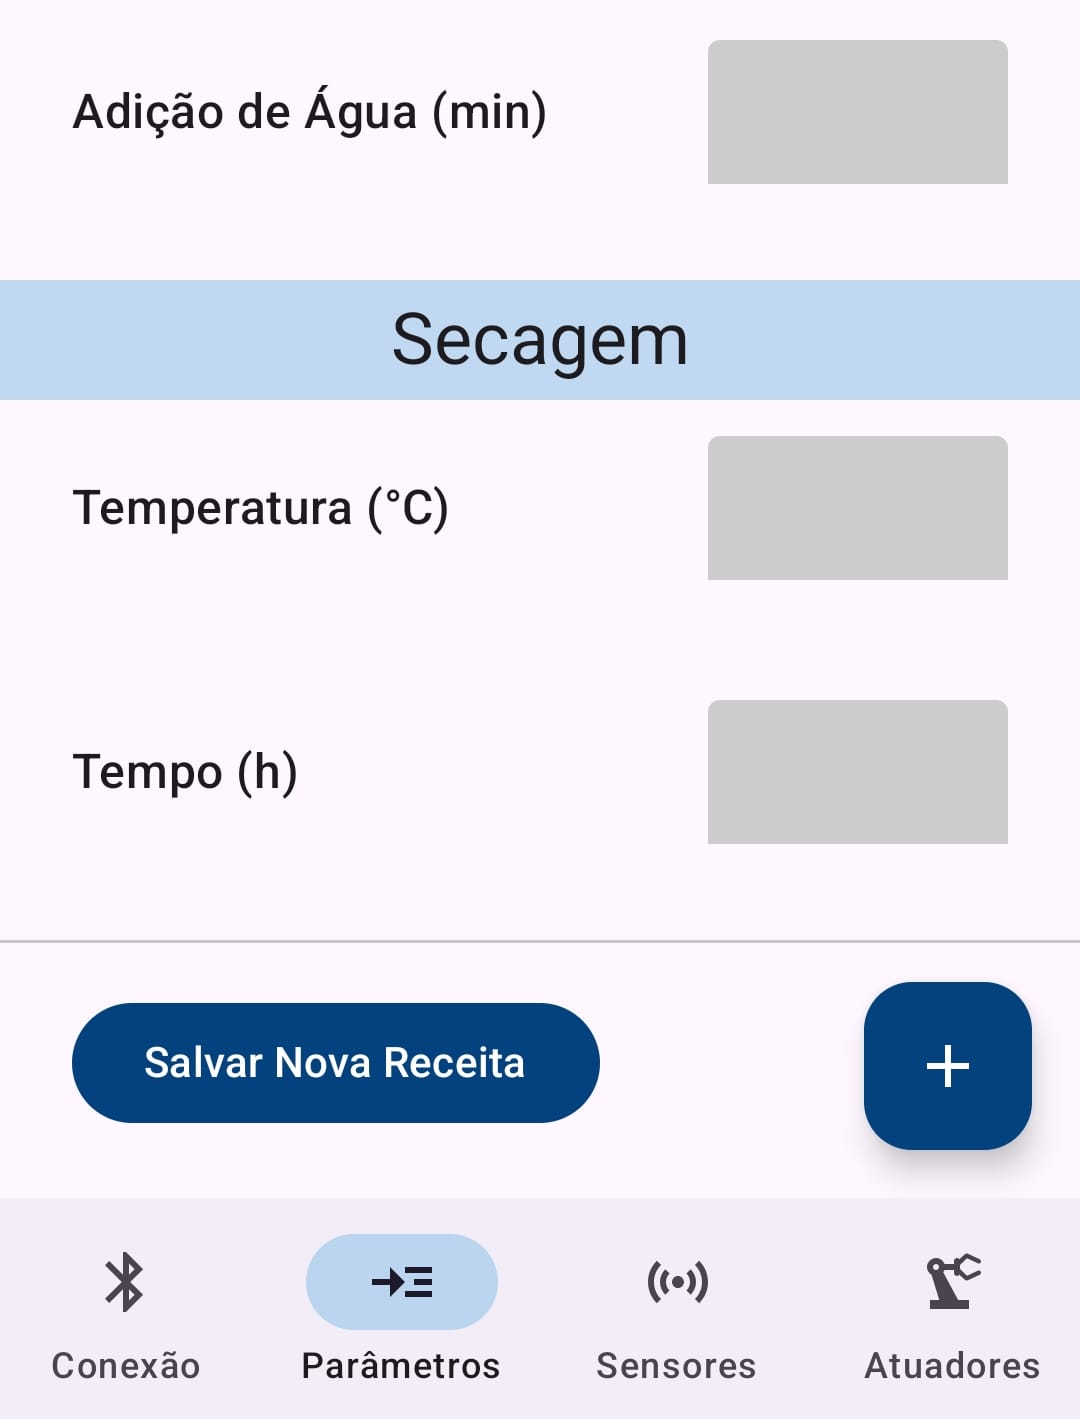
\includegraphics[width=0.32\textwidth]{save-recipe.jpeg}}
    \hfill
    \subfloat[Entrada de nome para salvamento de receita personalizada\label{fig:save-recipe-inputname}]{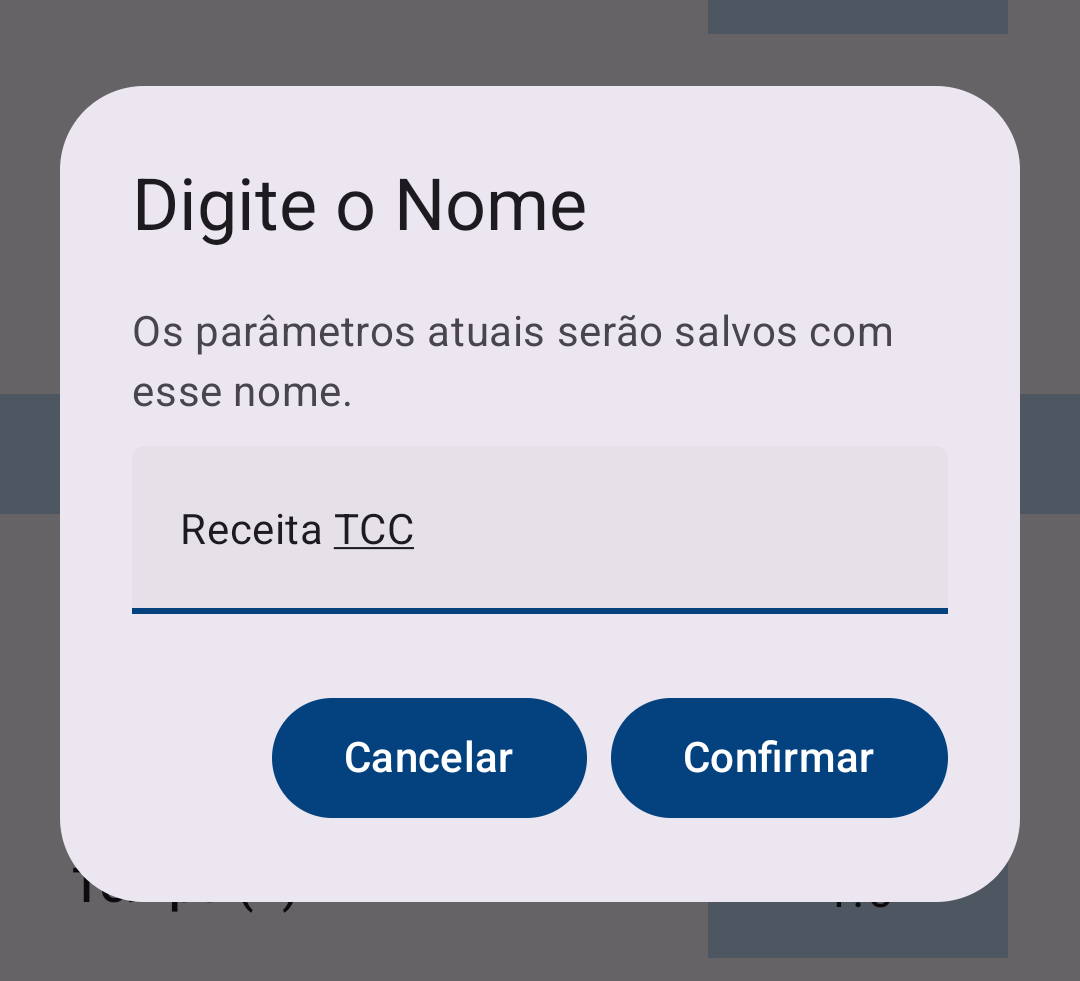
\includegraphics[width=0.32\textwidth]{save-recipe-inputname.png}}
    \hfill
    \subfloat[Seleção de receitas salvas\label{fig:select-recipe}]{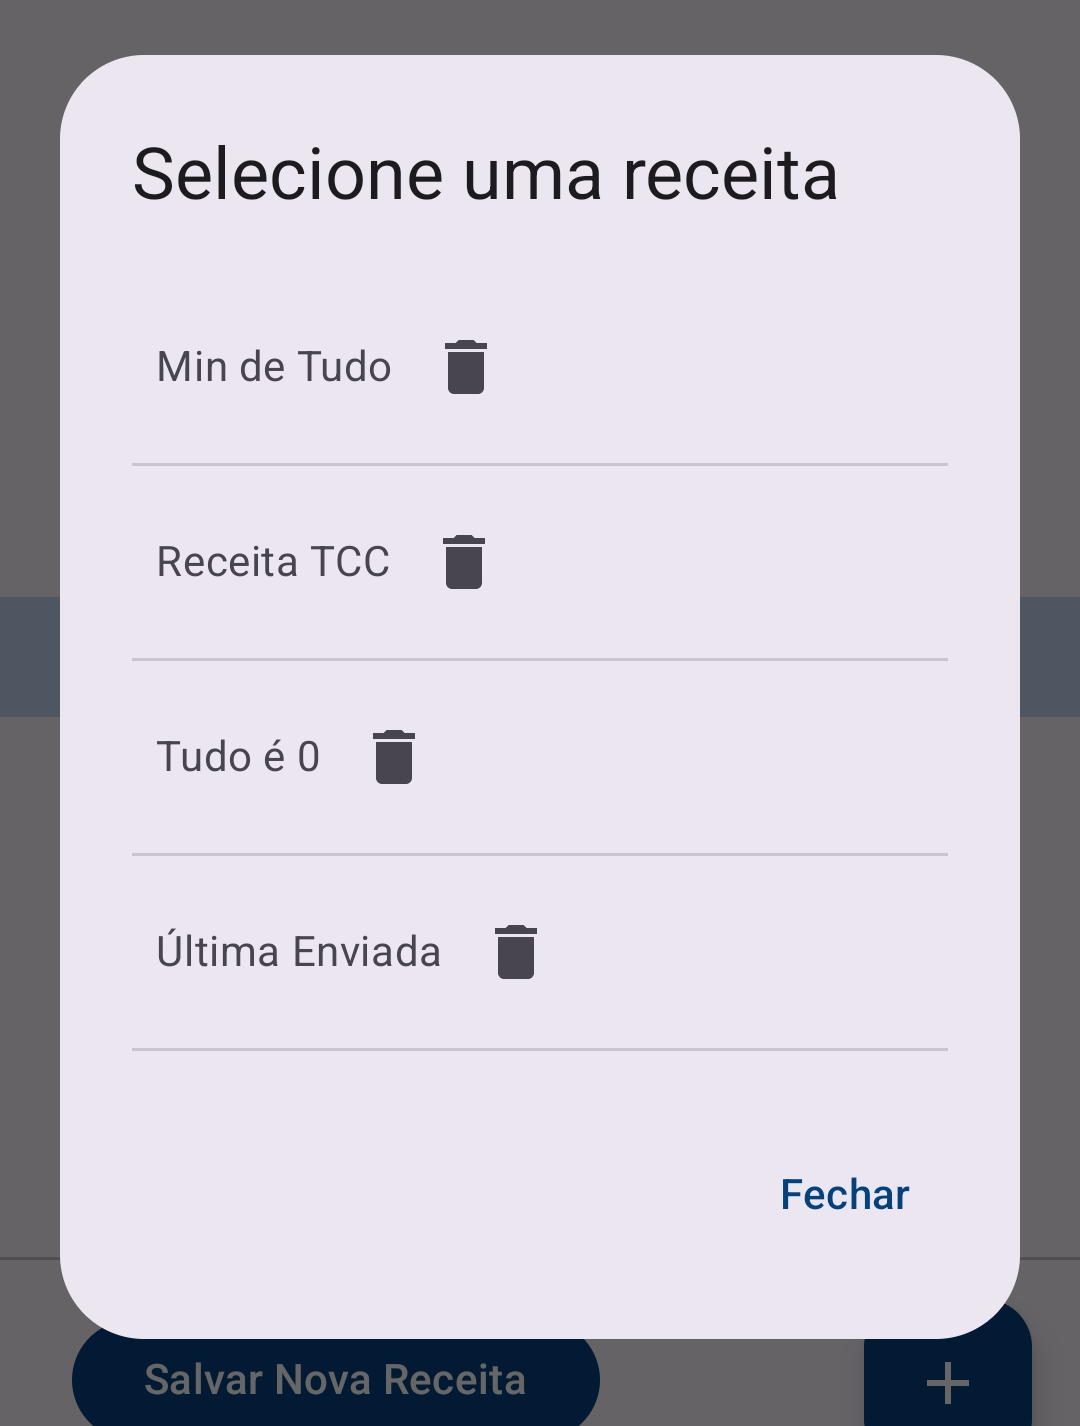
\includegraphics[width=0.32\textwidth]{select-recipe.png}}
    \hfill

    {\centering\footnotesize Fonte: Autoria própria.\par}

  \end{figure}

\subsection{Telas de Monitoramento: Sensores e Atuadores}\label{subsec:monitoramento}
As telas de sensores (\autoref{fig:sensors}) e atuadores (\autoref{fig:actuators}) cumprem função de monitoramento passivo, sem permitir interações diretas. A primeira exibe dados em tempo real de temperatura, umidade e concentração de CO$_2$, enquanto a segunda apresenta o estado operacional dos componentes físicos (válvulas, resistência, bomba de ar), com indicadores \textit{ON/OFF} gráficos. Ambas integram-se à \textit{BottomAppBar}, mantendo coerência na navegação e permitindo rápida alternância entre telas.

\begin{figure}[ht]
    \caption{Interface de sensores.}
    \label{fig:sensors}
    \centering
    \subfloat[Interface de sensores em modo desconectado\label{fig:sensores-off}]{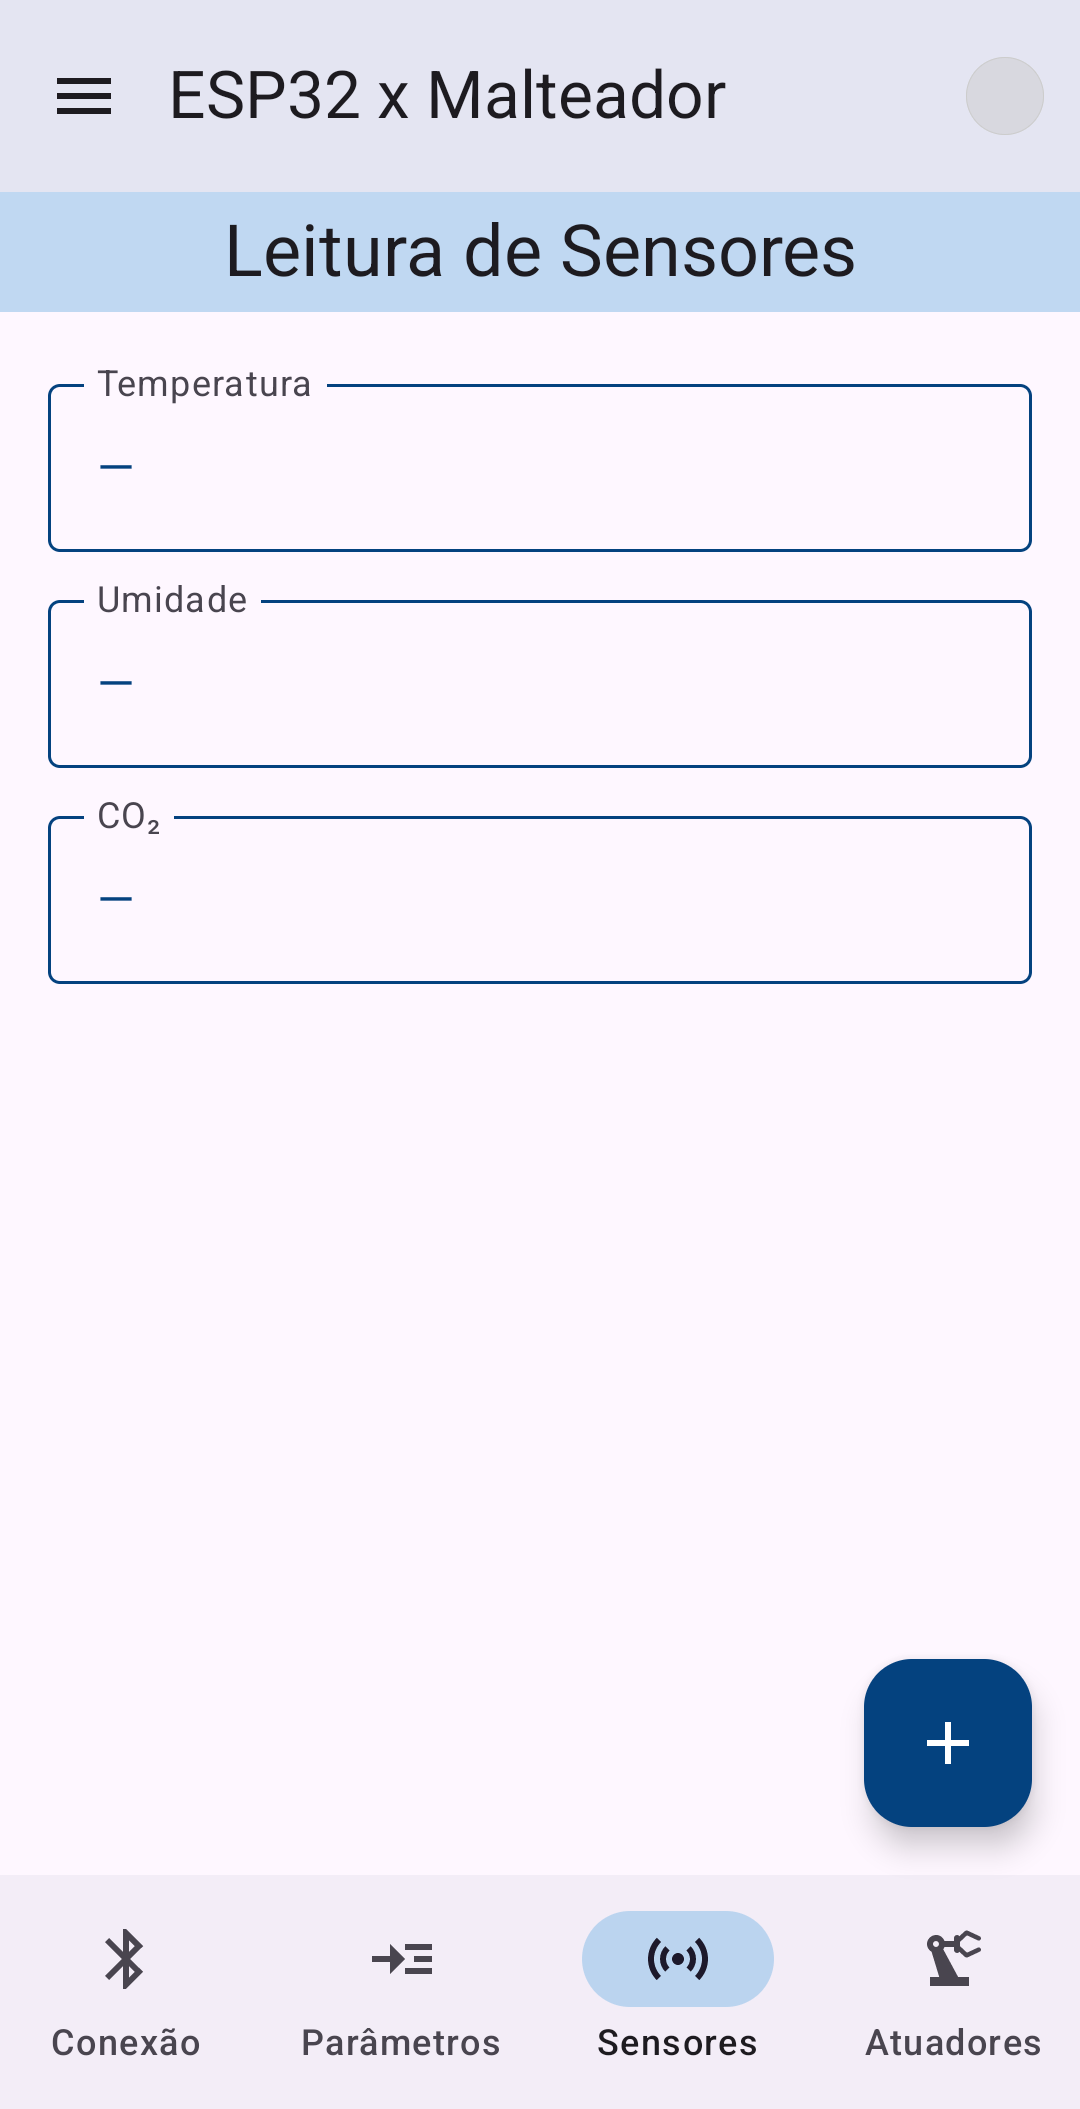
\includegraphics[width=0.3\textwidth]{sensores-off.png}}
    \hfill
    \subfloat[Interface de sensores em modo conectado\label{fig:sensores-on}]{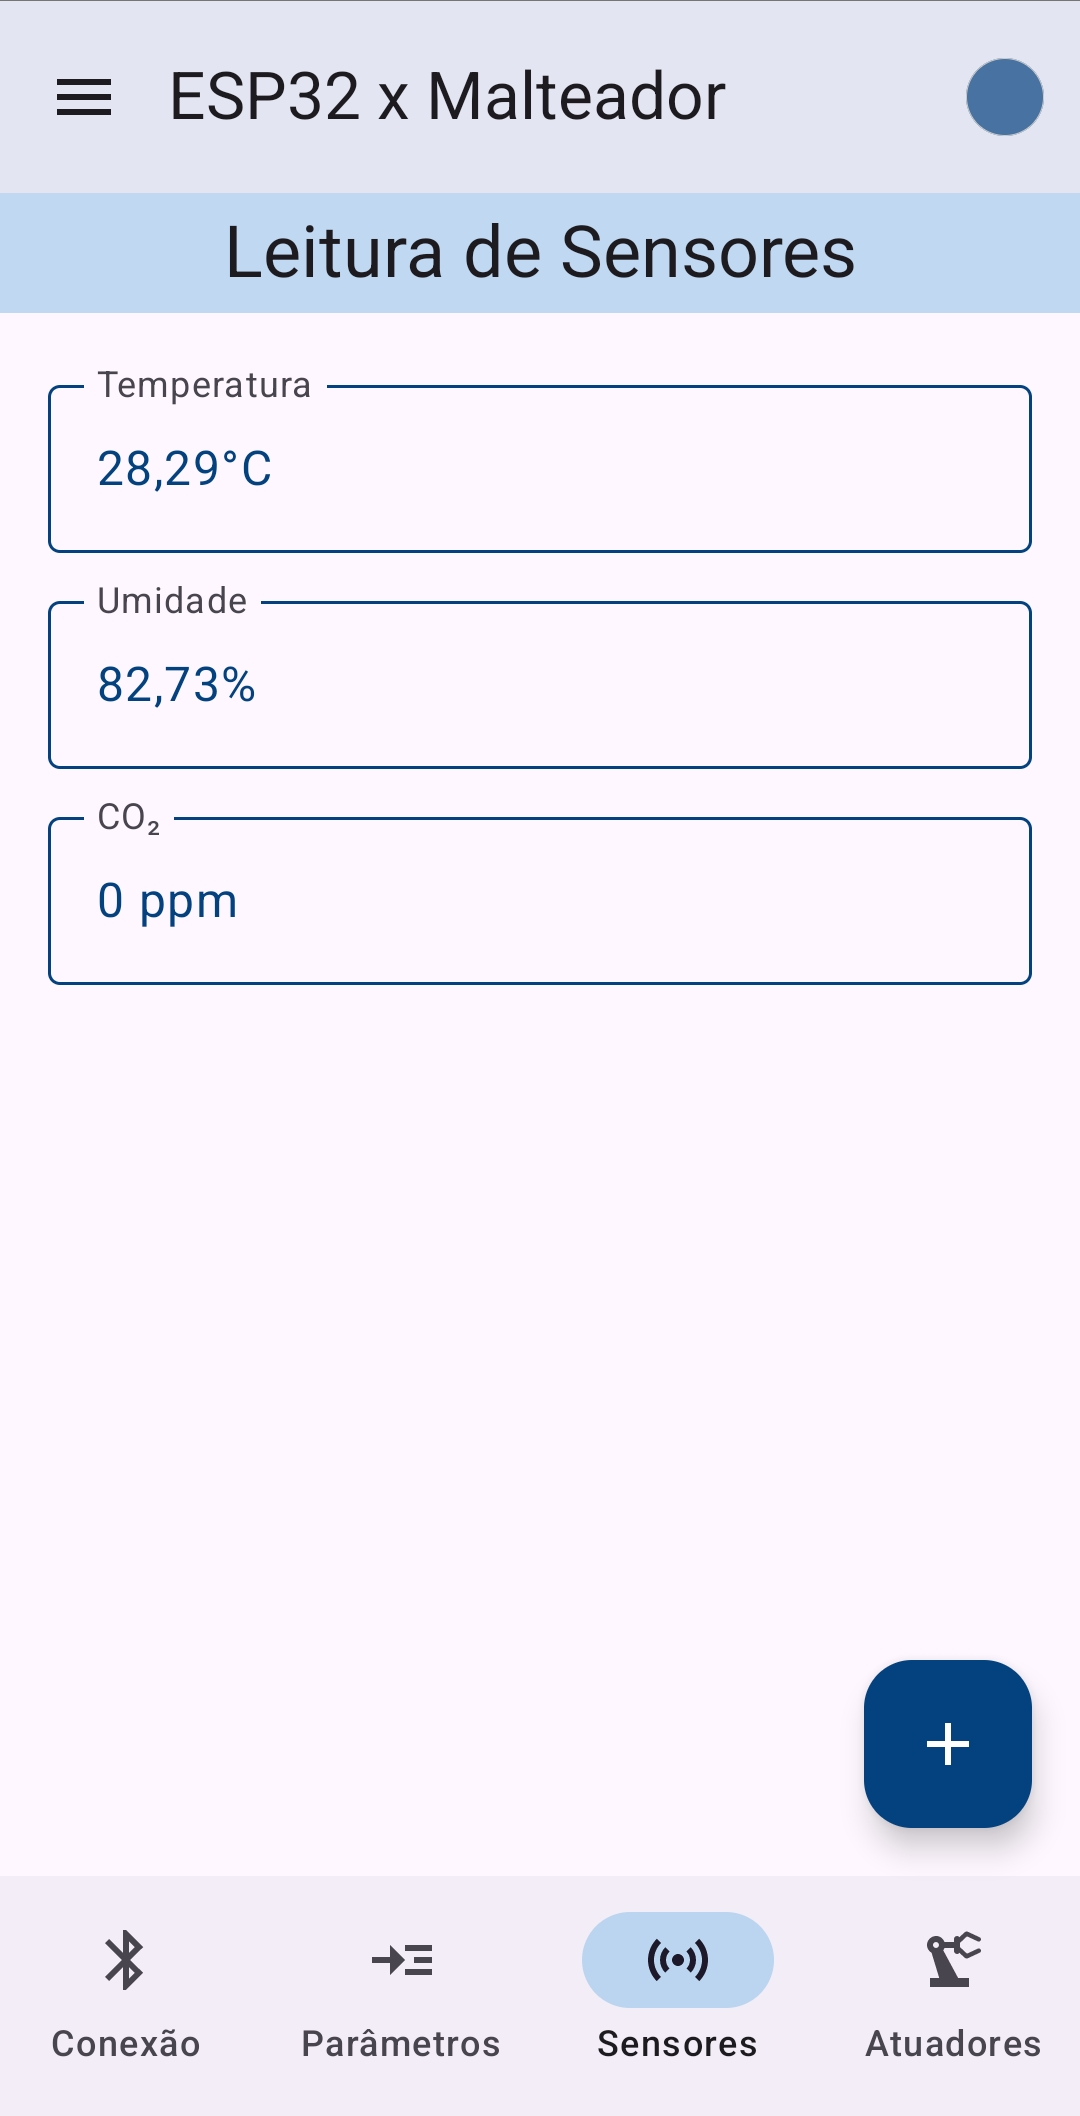
\includegraphics[width=0.3\textwidth]{sensores-on.png}}
    \hfill

    {\centering\footnotesize Fonte: Autoria própria.\par}

  \end{figure}

  \begin{figure}[ht]
    \caption{Interface de atuadores.}
    \label{fig:actuators}
    \centering
    \subfloat[Estado dos atuadores em modo desconectado\label{fig:atuador-off}]{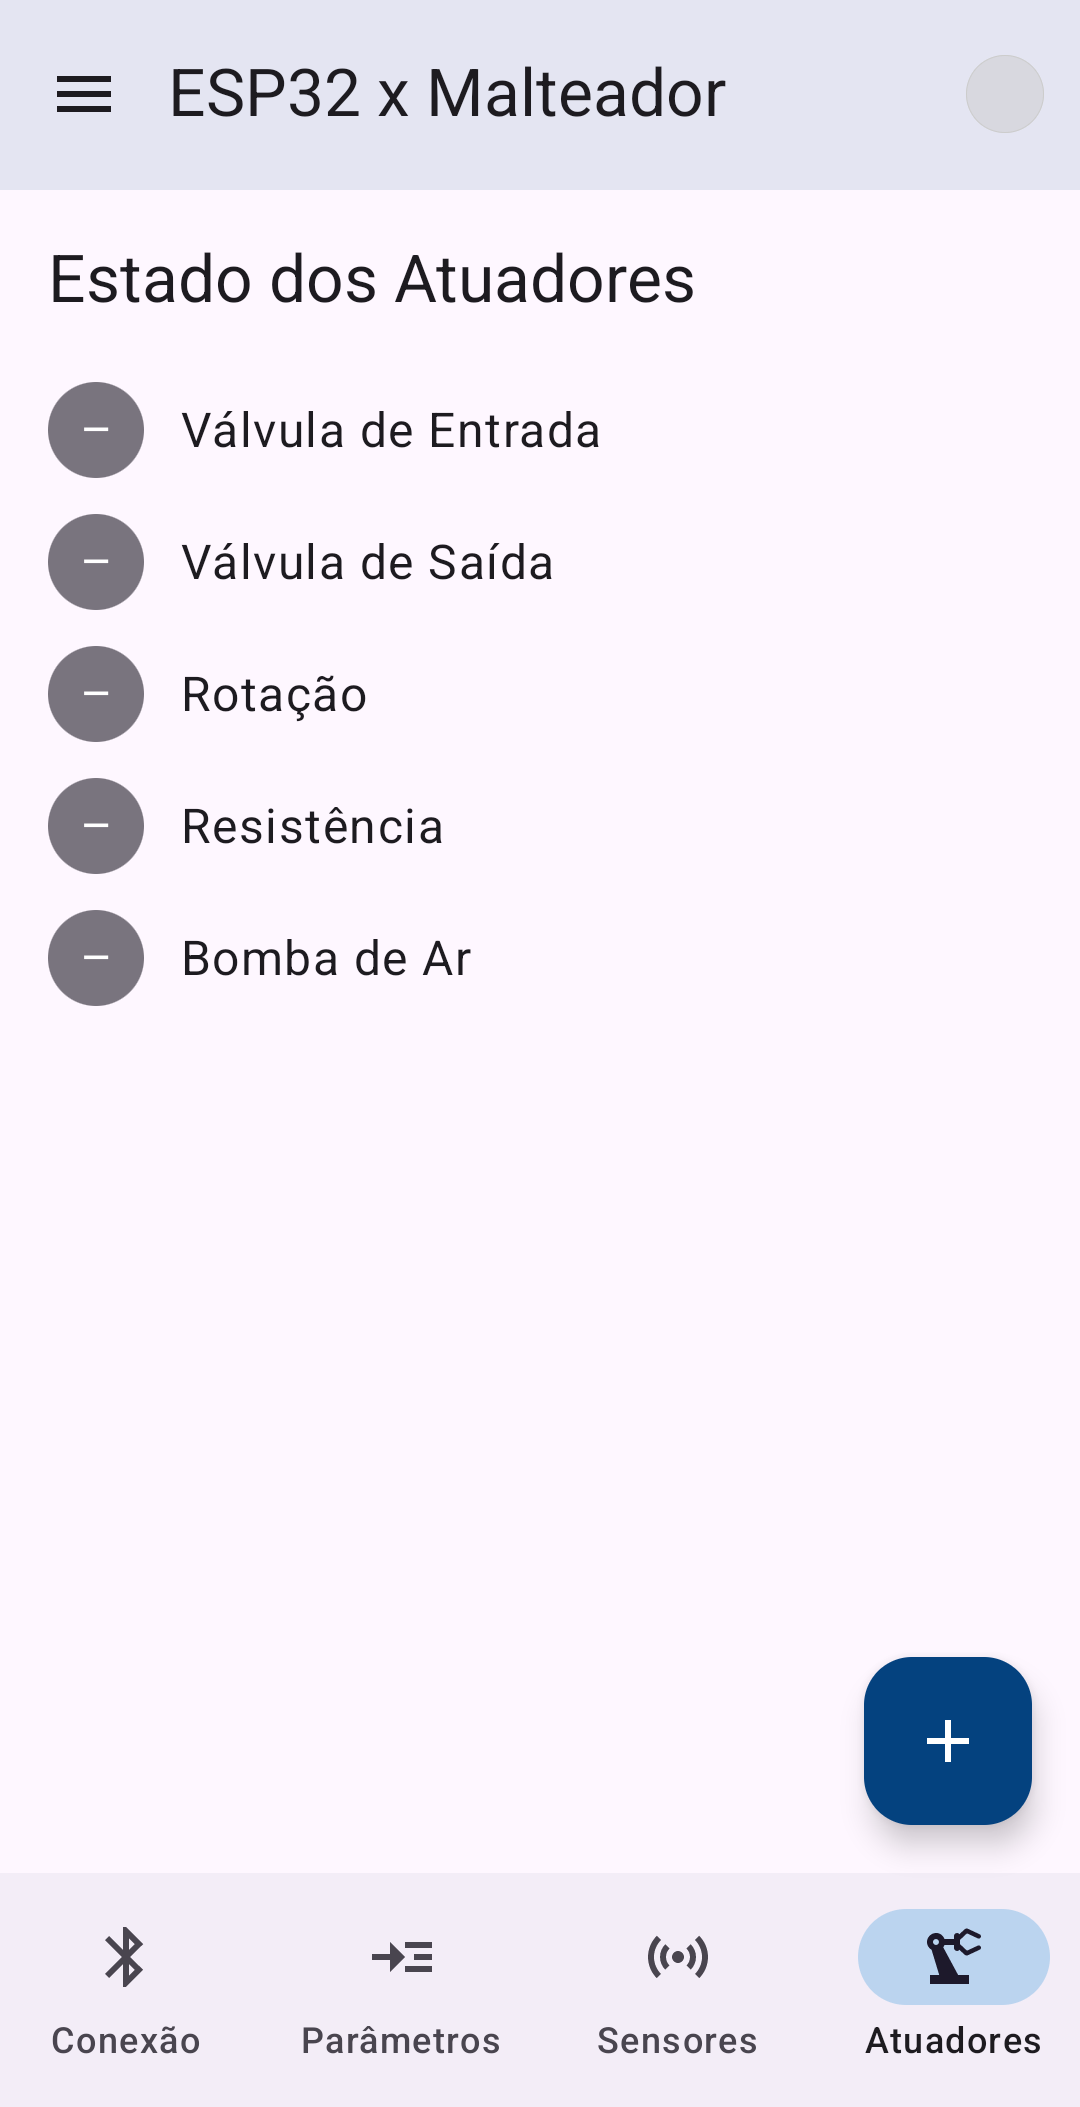
\includegraphics[width=0.3\textwidth]{atuador-off.png}}
    \hfill
    \subfloat[Interface de atuadores em modo conectado\label{fig:atuador-on}]{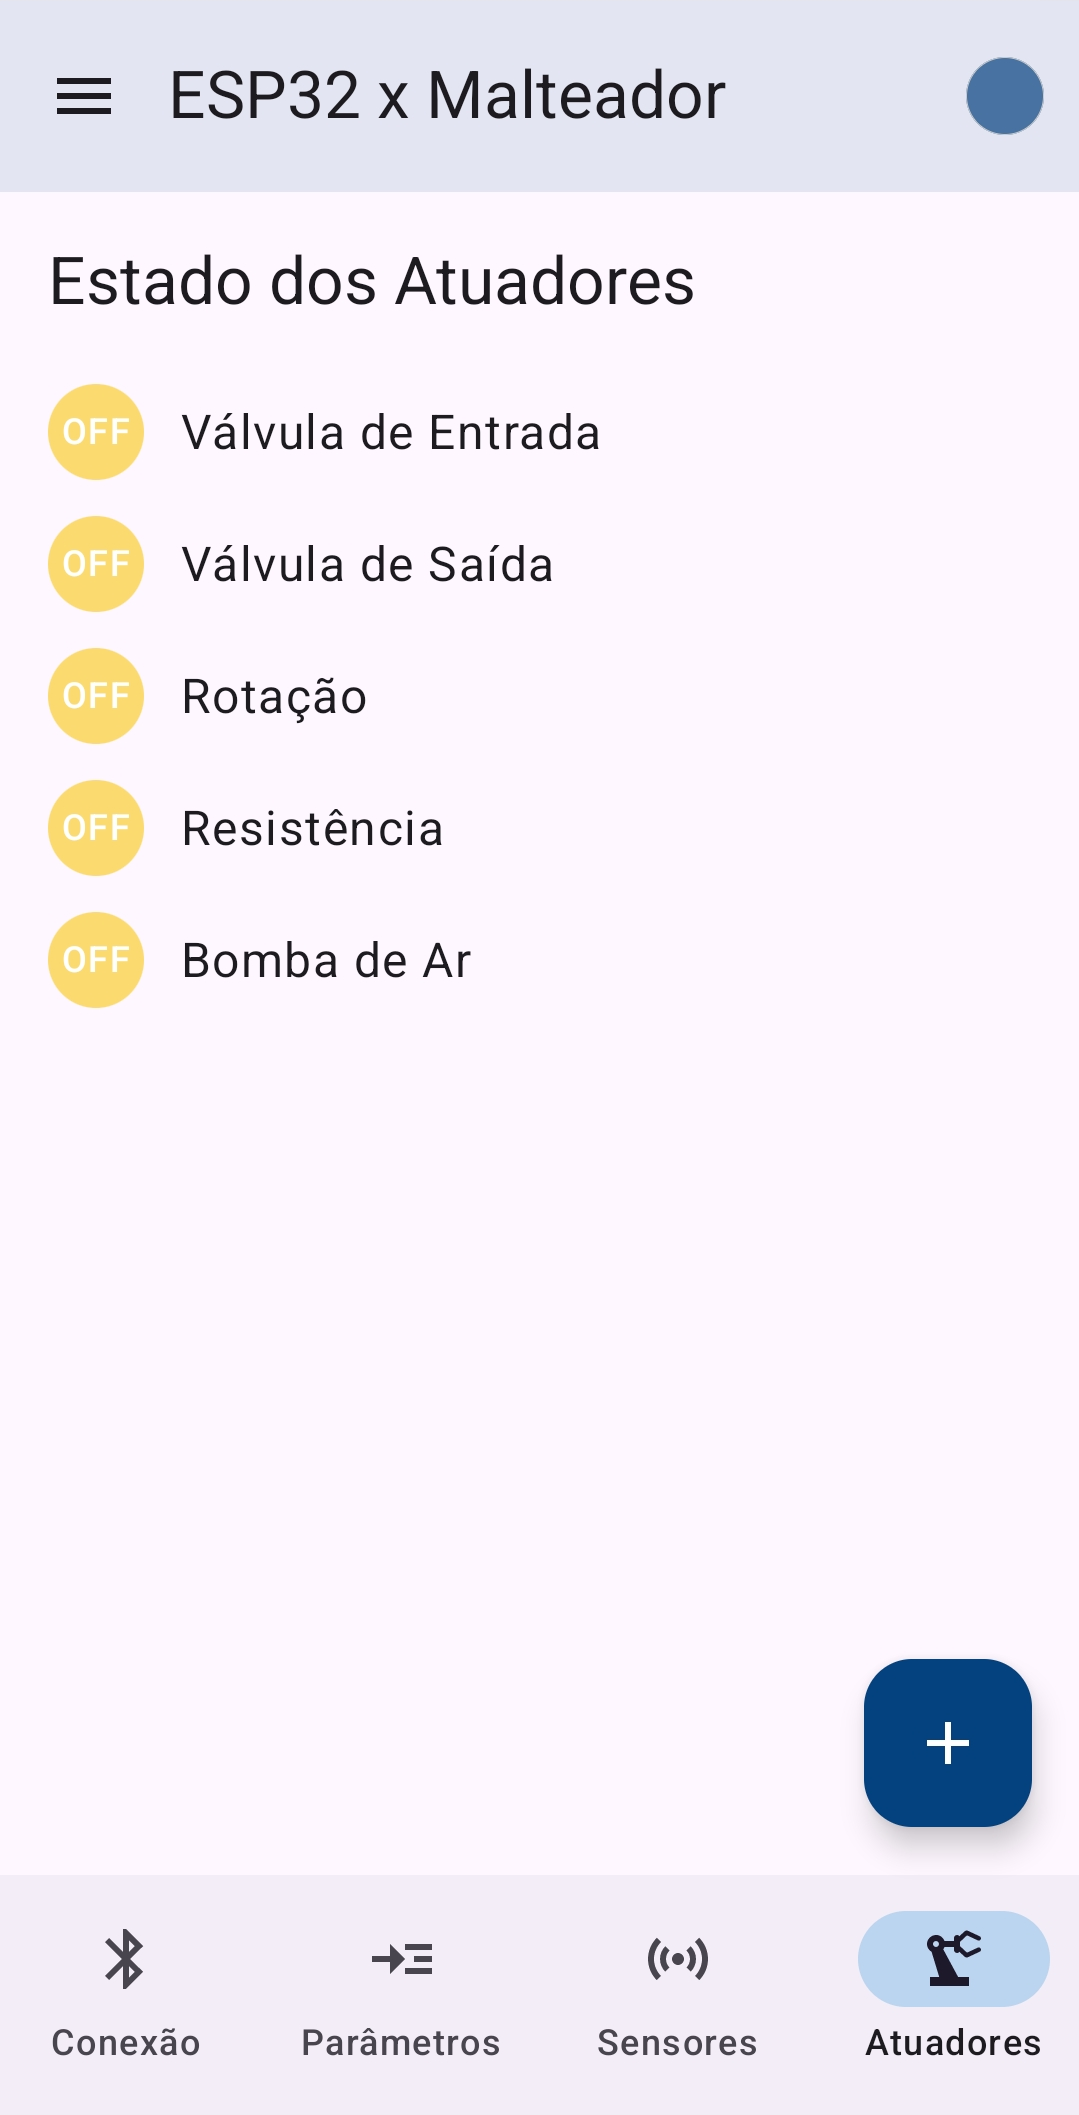
\includegraphics[width=0.3\textwidth]{atuador-on.png}}
    \hfill

    {\centering\footnotesize Fonte: Autoria própria.\par}

  \end{figure}

\section{Limitações e trabalhos futuros}

Embora a arquitetura de software esteja praticamente pronta, o presente trabalho apresenta limitações no que diz respeito à validação prática do sistema. O protótipo físico desenvolvido anteriormente, durante a IC, permanece incompleto em sua estrutura elétrica e nos componentes de automação, o que inviabilizou a realização de testes físicos com os controles implementados.
  
Como consequência, os testes foram realizados sem a ativação real dos atuadores. Os sensores AHT20 e ENS160 foram conectados ao sistema e realizaram leituras ambientais reais 
% (\autoref{fig:protoboard})
. O comportamento do código foi verificado por meio de mensagens no terminal, confirmando que os trechos responsáveis pelo acionamento de dispositivos estão sendo corretamente executados. Essa abordagem teve como objetivo validar a lógica de controle assíncrona e a estabilidade da comunicação via Bluetooth. A simulação demonstrou-se eficaz para comprovar o funcionamento da arquitetura em condições normais de operação.
  
% \begin{figure}[ht]
%     \centering
%     \caption{Protoboard montada com o (A) ESP32-C3 e (B) os sensores AHT20+ENS160 para validação das leituras.}
%     \label{fig:protoboard}
%     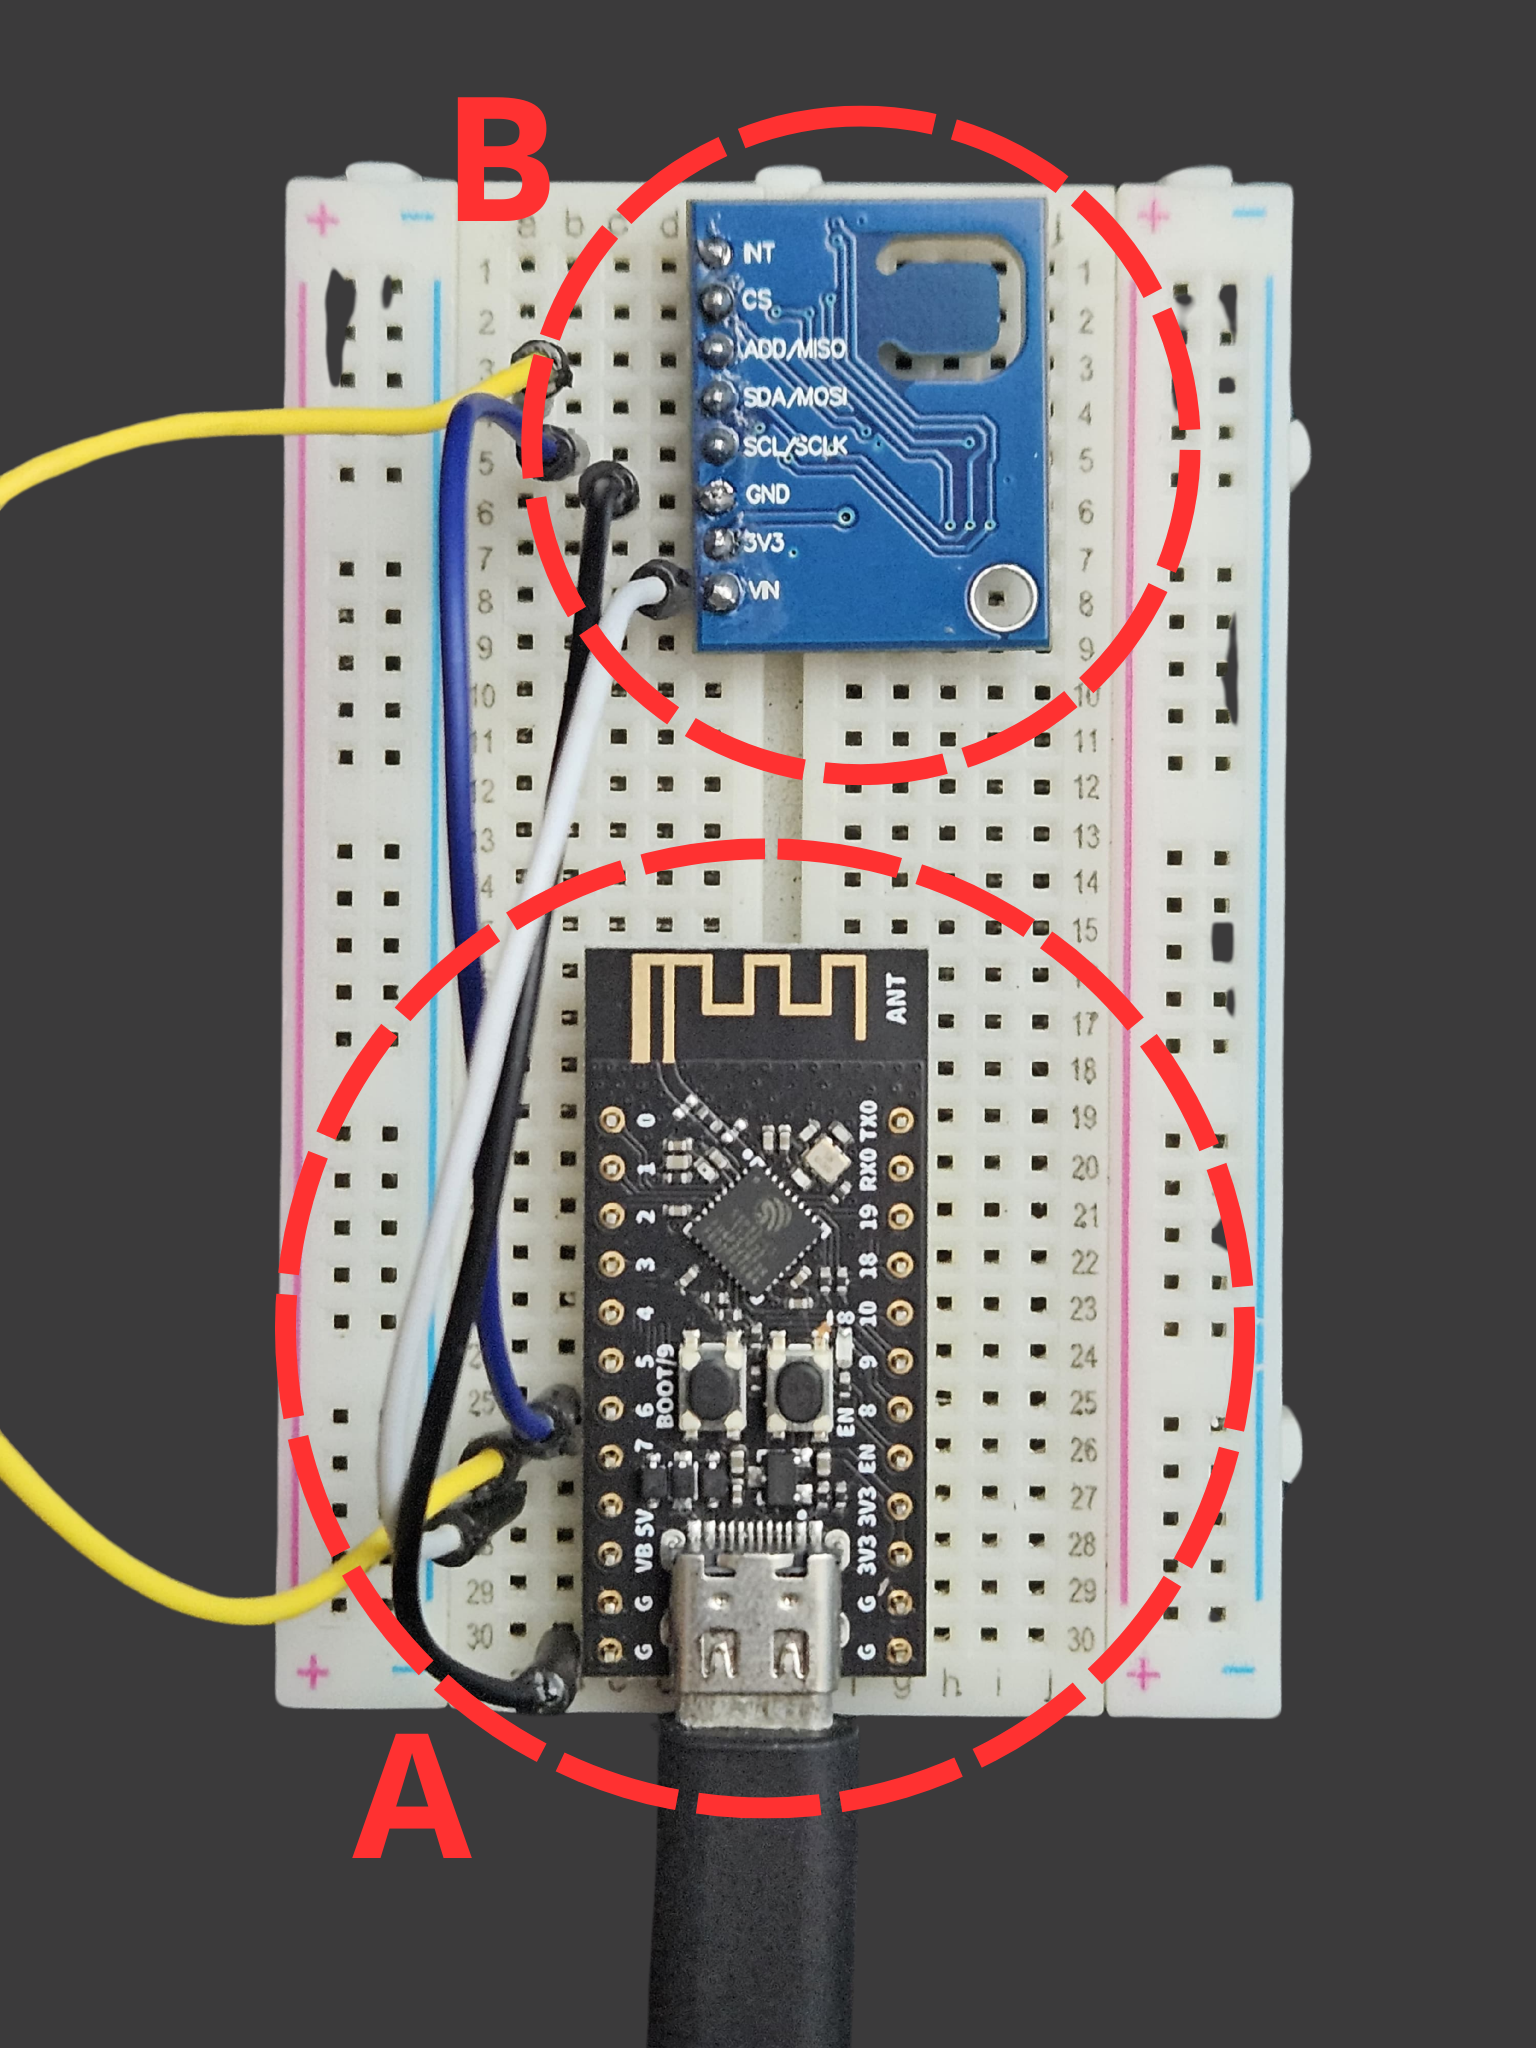
\includegraphics[width=0.8\textwidth]{protoboard.png}

%     {\centering\footnotesize Fonte: Autoria própria.\par}
%   \end{figure}
  
Para trabalhos futuros, recomenda-se:
  
  \begin{itemize}
      \item Finalização do protótipo físico com sensores e atuadores totalmente integrados;
      \item Avaliação da eficiência do sistema em testes com diferentes perfis de malteação;
      \item Implementação de novos recursos, como controle de torrefação e exportação de dados históricos.
  \end{itemize}
  \chapter[Conclusão]{Conclusão}

Este trabalho apresentou o desenvolvimento de um sistema de automação para controle do processo de malteação em escala laboratorial, com base em uma arquitetura composta por \textit{firmware} para o microcontrolador \textit{ESP32-C3} e um aplicativo \textit{Android}. A proposta surgiu da necessidade identificada no \textit{LACEMP-IFES} por uma solução de baixo custo e com potencial didático, voltada ao estudo controlado da malteação em climas quentes.

O \textit{firmware} foi estruturado com lógica assíncrona, permitindo a execução simultânea de múltiplas tarefas, como leitura de sensores, controle de etapas e comunicação via \textit{Bluetooth Low Energy}. Por sua vez, o aplicativo \textit{Android}, desenvolvido em \textit{Kotlin}, adotou uma arquitetura modular em camadas, com funcionalidades que incluem envio de parâmetros, monitoramento em tempo real e gerenciamento de receitas.

Dentro do escopo estabelecido, os objetivos propostos foram alcançados: a comunicação \textit{BLE} entre os dispositivos foi implementada com sucesso, os algoritmos de controle das etapas de maceração, germinação e secagem foram desenvolvidos e validados por meio de simulações, e todo o código foi documentado e disponibilizado em repositórios públicos.

Embora validada por simulações, a solução não foi testada com o protótipo físico em funcionamento, uma vez que sua montagem completa e integração eletromecânica estavam fora do escopo deste trabalho. Assim, os testes com sensores e atuadores reais permanecem como uma etapa futura necessária para avaliar a performance prática da malteação realizada no equipamento.

Dessa forma, o trabalho cumpriu seu papel, entregando uma base funcional e bem documentada para o controle digital do processo. Apesar da ausência de testes com \textit{hardware} real, os resultados obtidos por simulação demonstram a viabilidade da proposta e oferecem um ponto de partida concreto para desenvolvimentos futuros.
      
  % --------------------------------------------------- %
  % ELEMENTOS POS-TEXTUAIS %
  % --------------------------------------------------- %
  \postextual
  
  % Referencias Bibliográficas
  \bibliographystyle{abntex2-alf} % Autor-Data
  \bibliography{bibliografia}
    
  % Apêndices
  \begin{apendicesenv}
    \input{pos_textuais/apendice.tex}
  \end{apendicesenv}

  % Anexos
  \begin{anexosenv}
    \input{pos_textuais/anexo.tex}
    \input{pos_textuais/easyreview.tex}
  \end{anexosenv}

  % Índice Remissivo
  \phantompart
  \printindex

\end{document}